
\section{Results}

{
    This section will present and discuss the results using the best models found and the results of the experiments explained at the previous section. 
}

{
    The results are based on 150 frames (10 seconds) from the video with a tray and 87 ants. 
    This source video was not used neither in the training or validation of any subsystem of the tracking model. 
    The annotations where made as accurately as possible using \ac{CVAT}.
}

\needspace{0.25\textheight}
\subsection{Detection Training}


{
    The YOLOv8 training curves, are a visual representation that serves as a snapshot of the model development.
}

\begin{figure}[!p]
	\centering
	\begin{subfigure}[b]{\textwidth}
		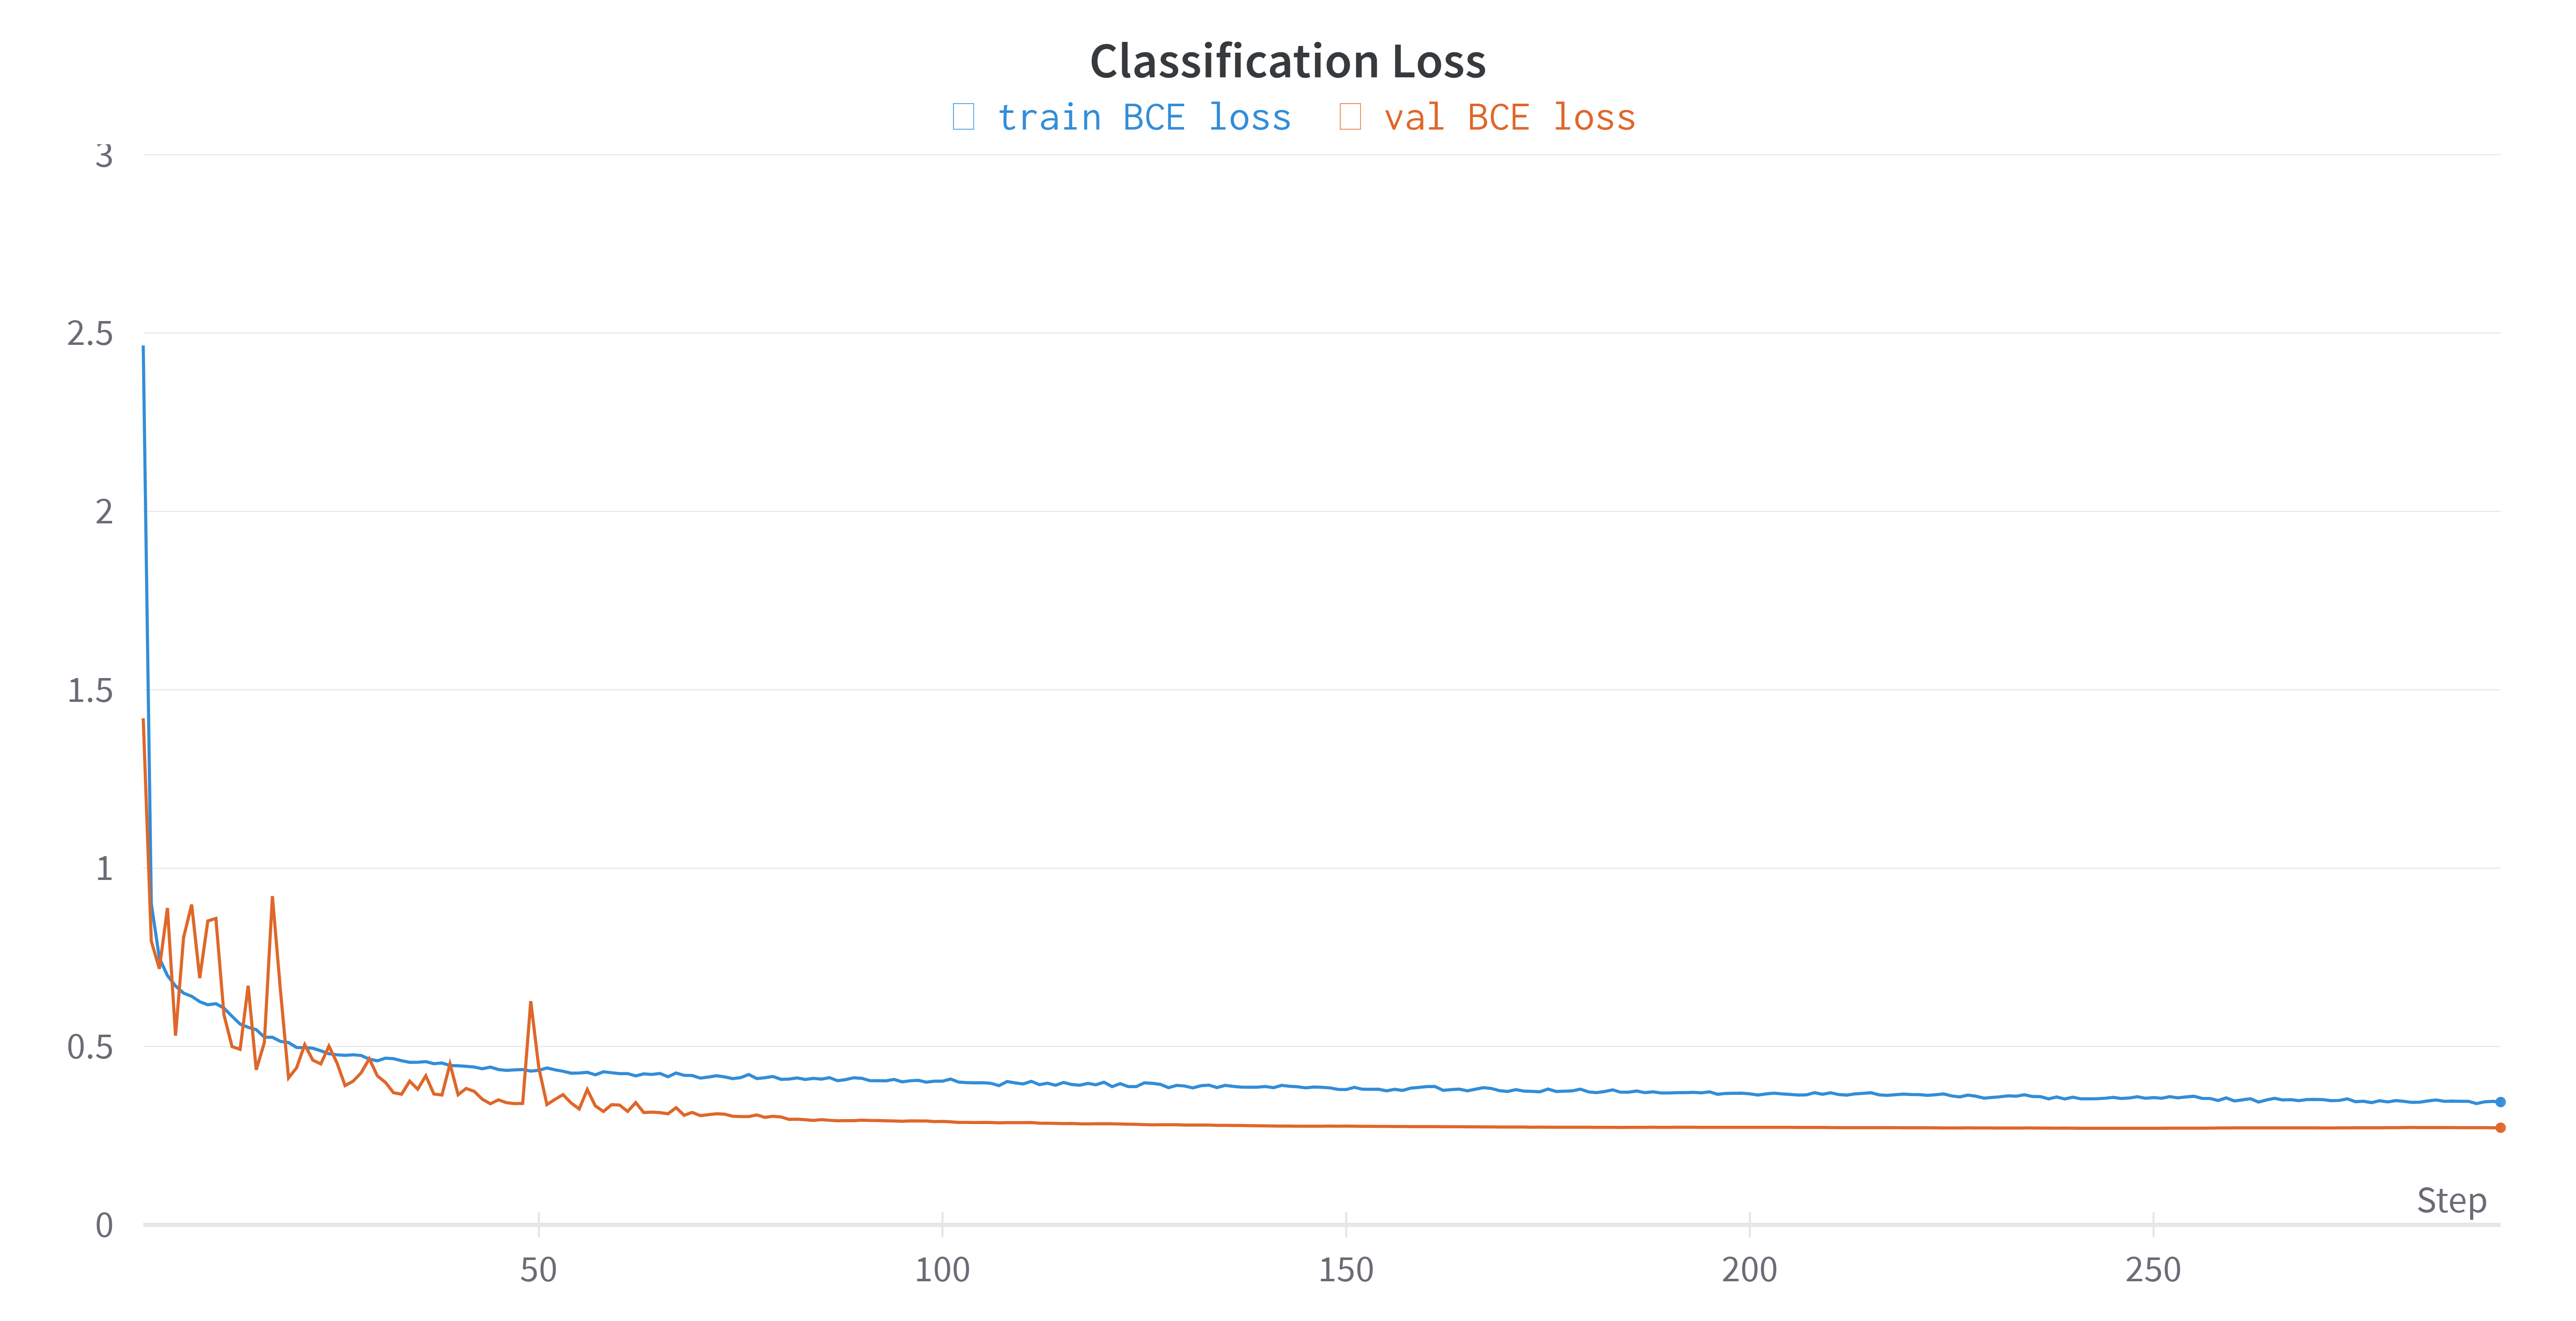
\includegraphics[width=\textwidth]{figures/06_results/ClassLossDetector.png}
		\caption{\footnotesize{Train and validation curves for the class classification loss.}}
		\label{fig:detector_class_loss}
	\end{subfigure}
	\begin{subfigure}[b]{\textwidth}
		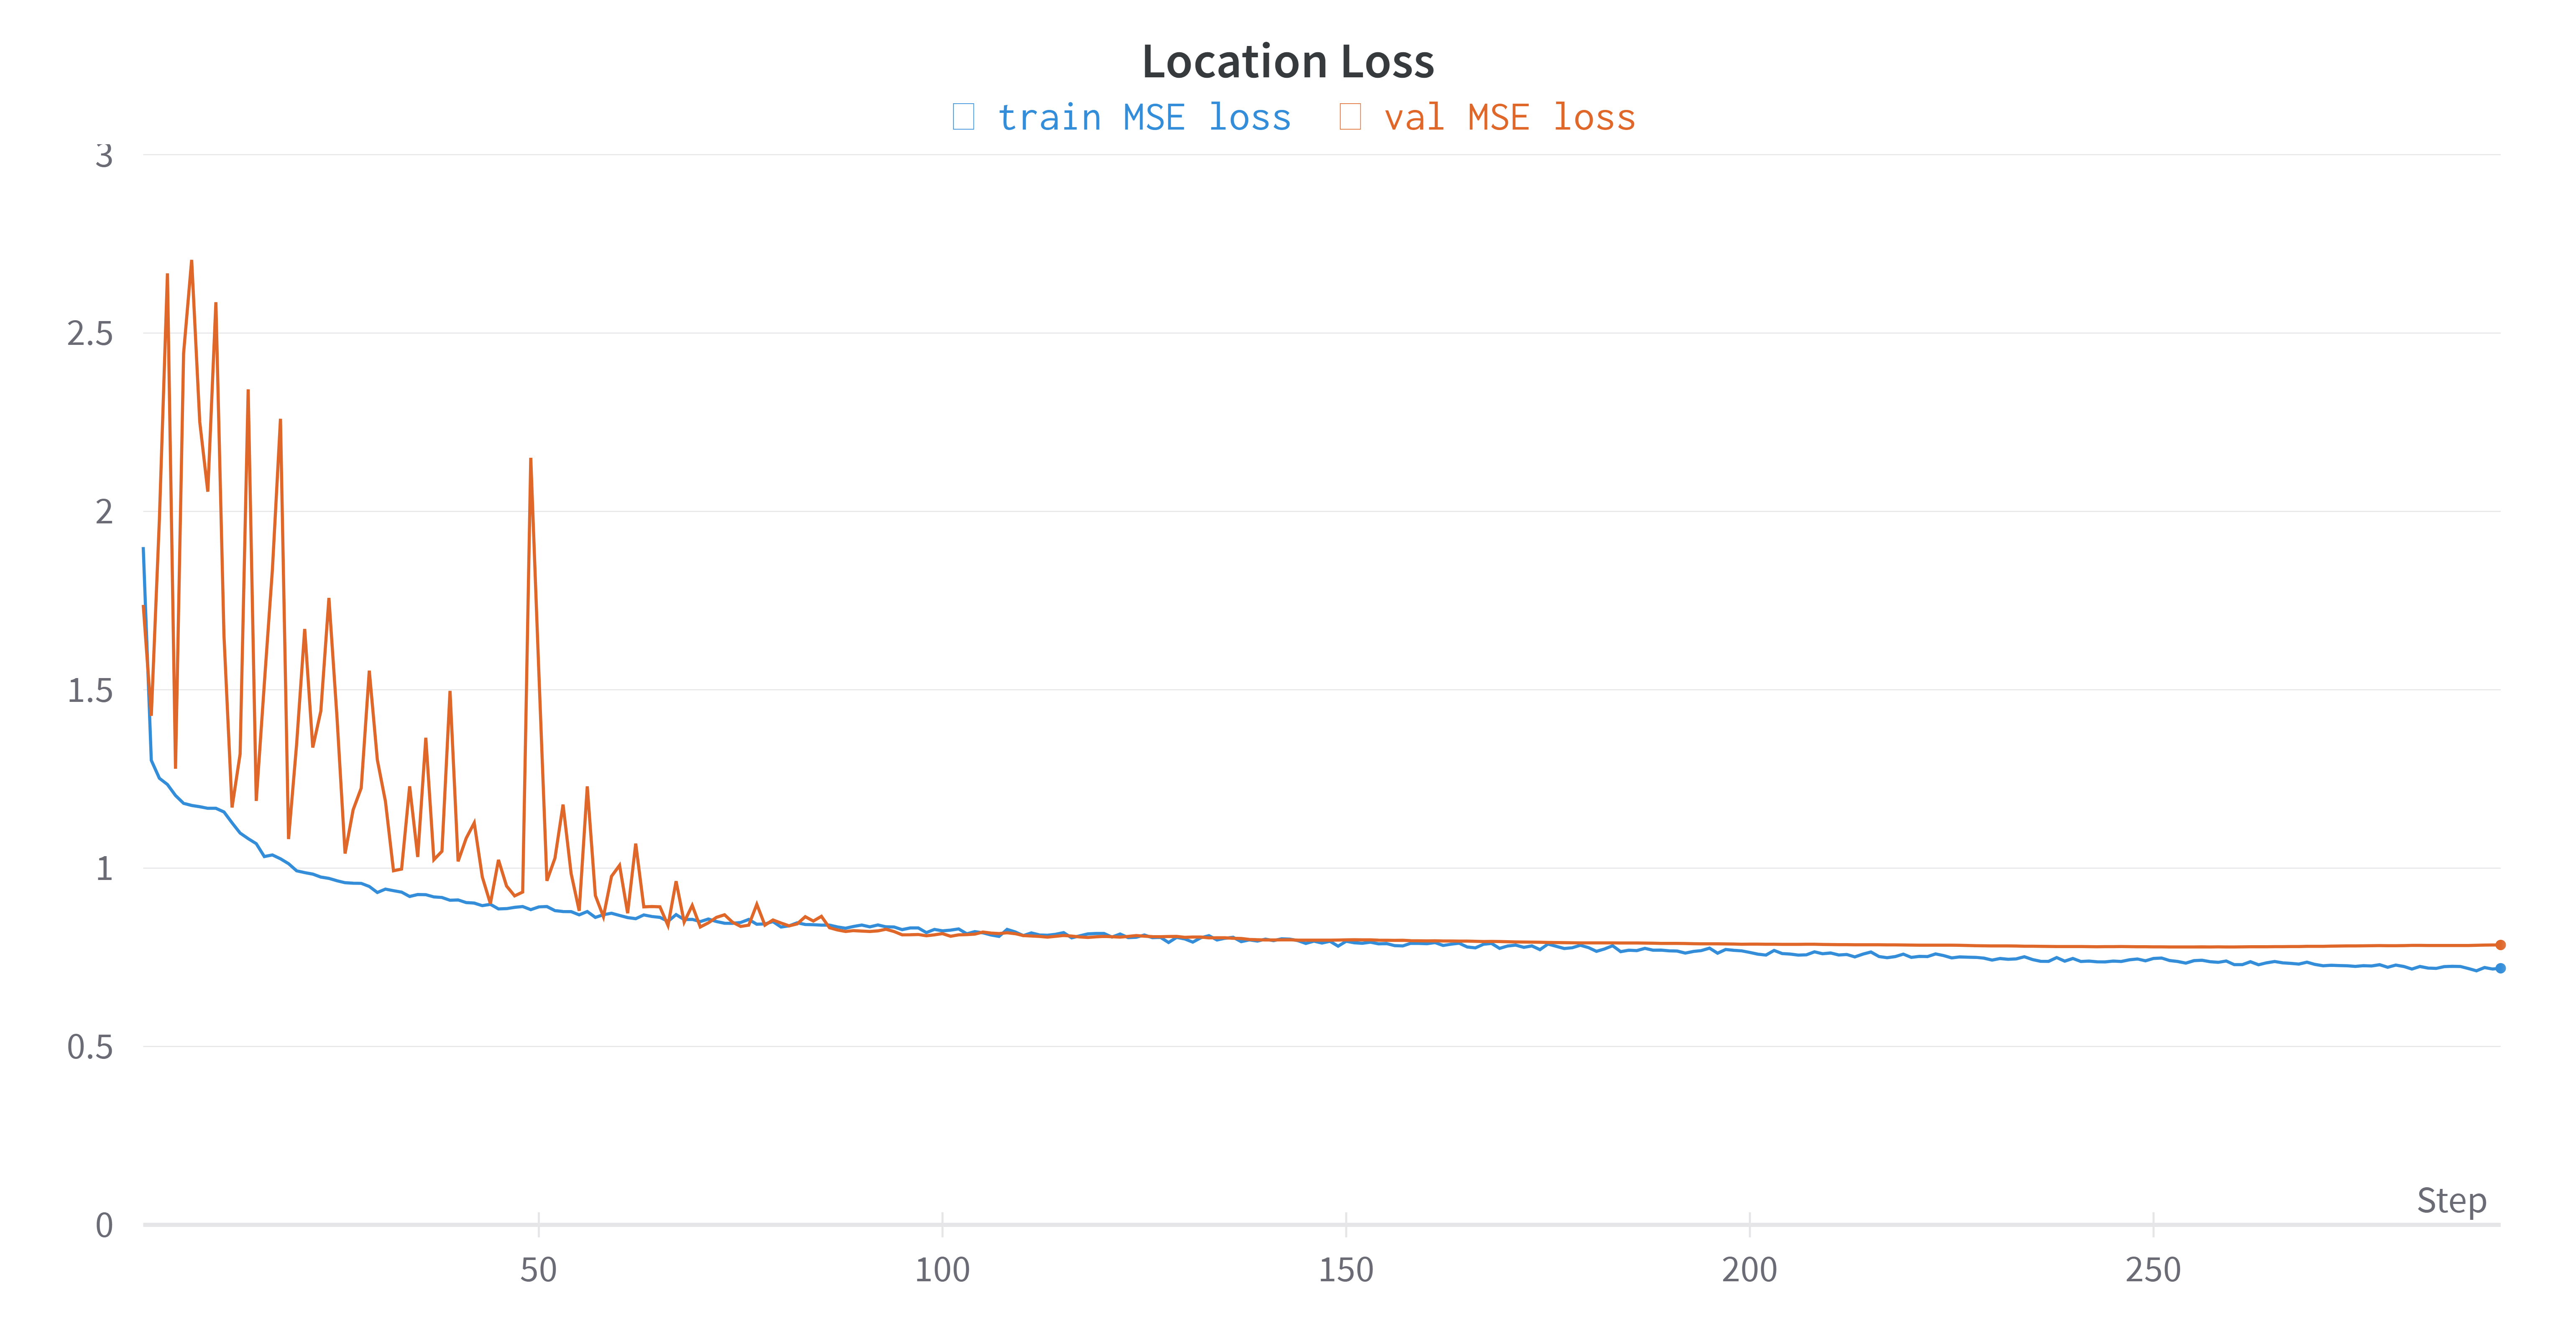
\includegraphics[width=\textwidth]{figures/06_results/LocationLossDetector.png}
		\caption{\footnotesize{Train and validation curves for the object location loss.}}
		\label{fig:detector_location_loss}
	\end{subfigure}
	
	\caption[Train and validation loss curves of YOLOv8]{\footnotesize{Train and validation loss curves of YOLOv8.}}
	\label{fig:yolov8 train curves}
\end{figure}

{
    From the curves on Figure \ref{fig:yolov8 train curves}, it can be seen the learning process starts fluctuating only on validation because the model is not optimized and the validation contains some randomness. 
	As the training advances, the validation curve stabilizes and slowly improves until the epoch 243; at the epoch 293 (of a maximum of 500) the trainer program early stopped the training. 
    The training ended successfully without overfitting.
}

%\begin{figure}[!p]
%    \centering
%    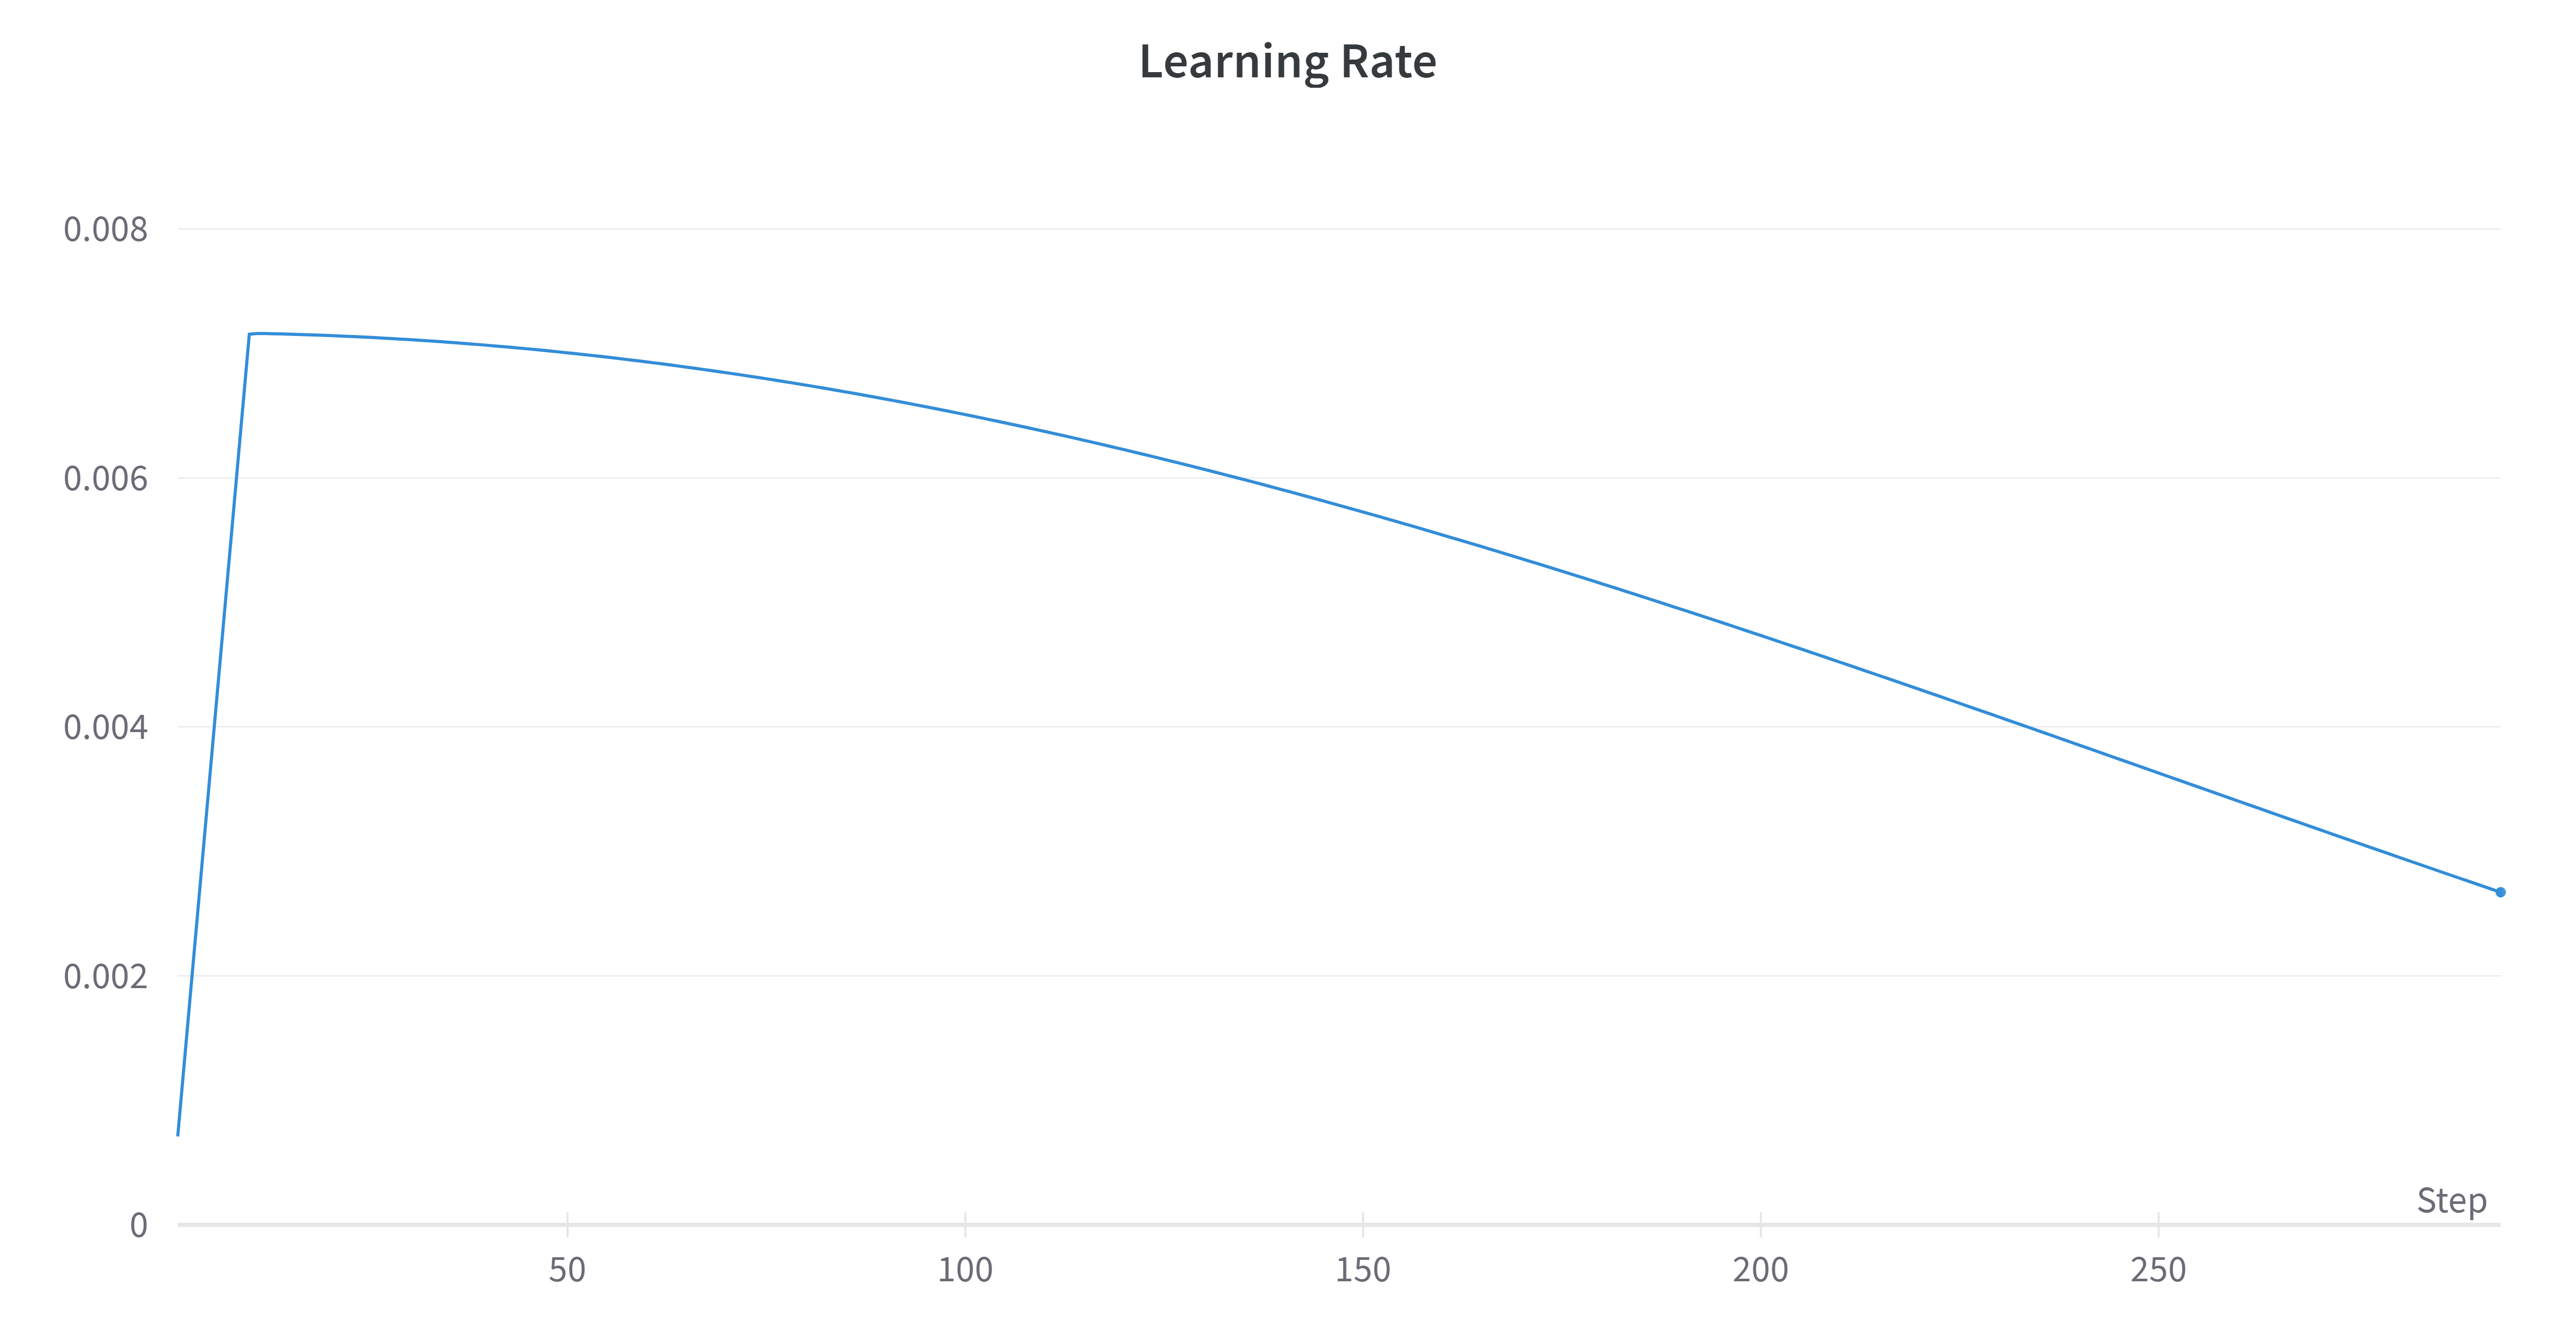
\includegraphics[width=0.45\textwidth]{figures/06_results/LearningRateDetector.png}
%    \caption[Learning rate curve of YOLOv8]{\footnotesize{Learning rate curve for the YOLOv8 training.}}
%    \label{fig:detector_learning_rate}
%\end{figure}

{
    Additionally, it was seen that, when adding more difficult data, the model reached a better solution\footnote{This result is valid because the ampliation of the validation dataset increased the difficulty (from a dataset of only one ant to a dataset with multiple ants interacting in groups), however, it would be better to repeat the curves with a unique version of the validation dataset.} on the increased dataset. 
    The validation \ac{mAP}@50-95 curves on Figure \ref{fig:validation mAP50-95} illustrates this statement, where both curves have similar shapes but different endpoints.
}

\begin{figure}[!p]
	\centering
	\begin{subfigure}[]{0.45\textwidth}
		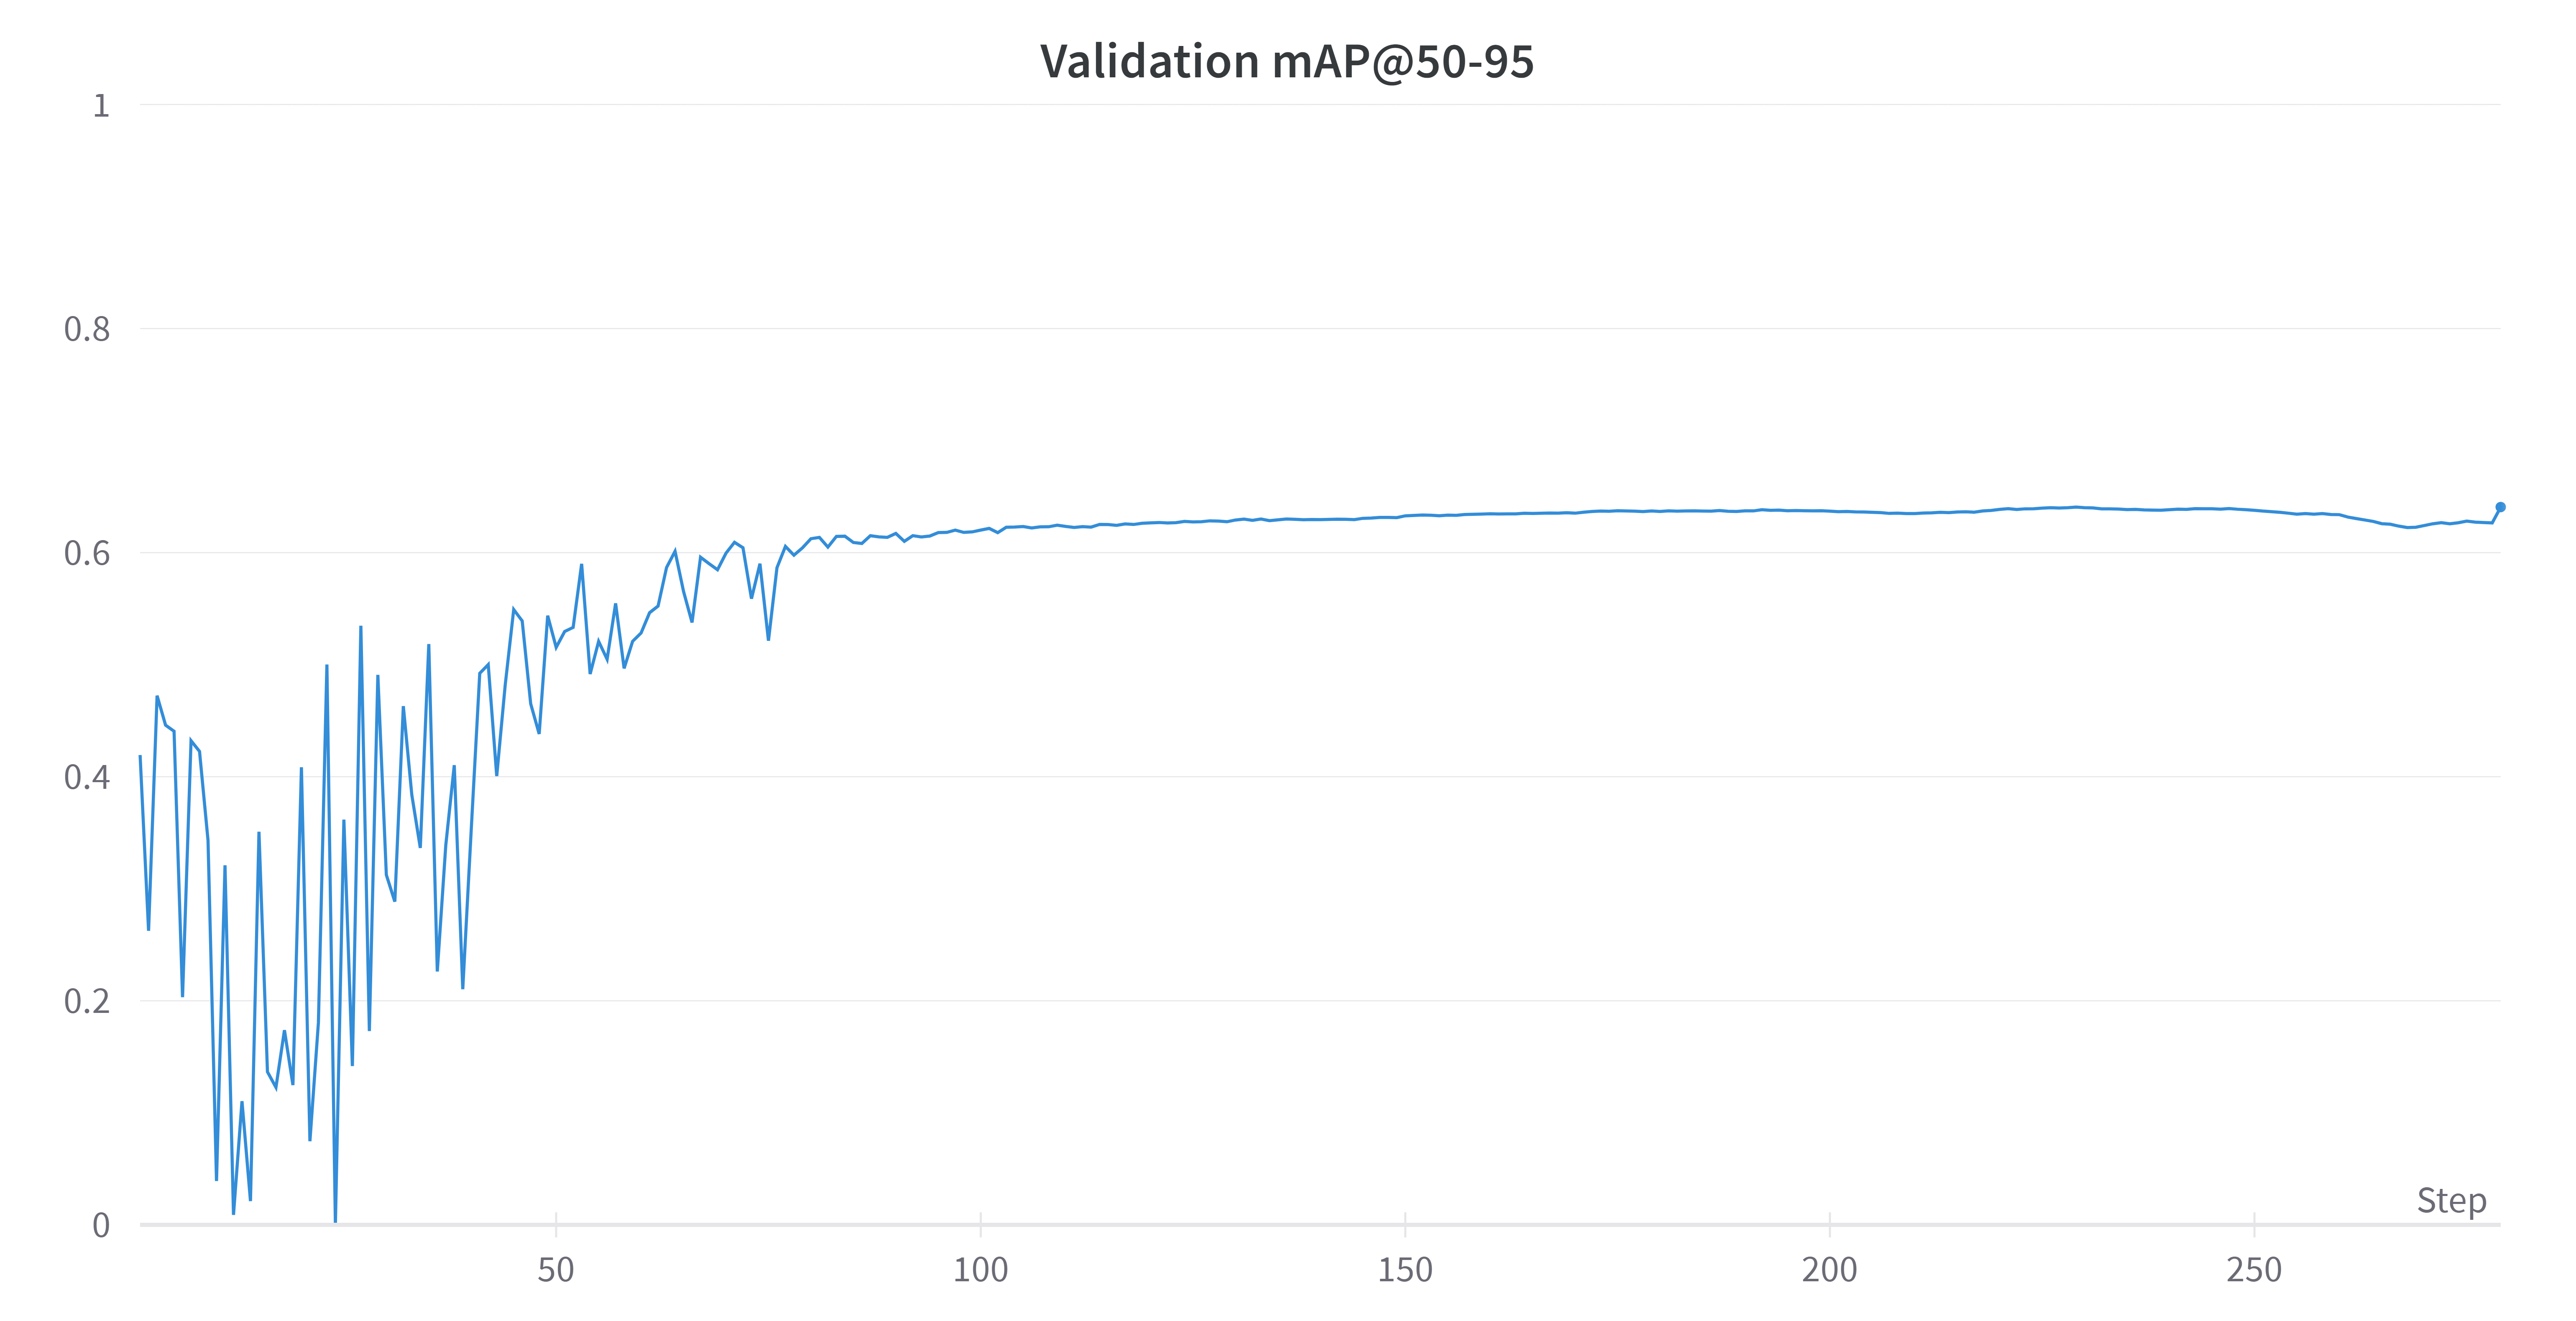
\includegraphics[width=\textwidth]{figures/06_results/mAP5095DetectorInitial.png}
		\caption{\footnotesize{Validation mAP@50-95 curves of YOLOv8 with the smaller dataset.}}
		\label{fig:validation mAP50-95 Initial}
	\end{subfigure}
	\begin{subfigure}[]{0.45\textwidth}
		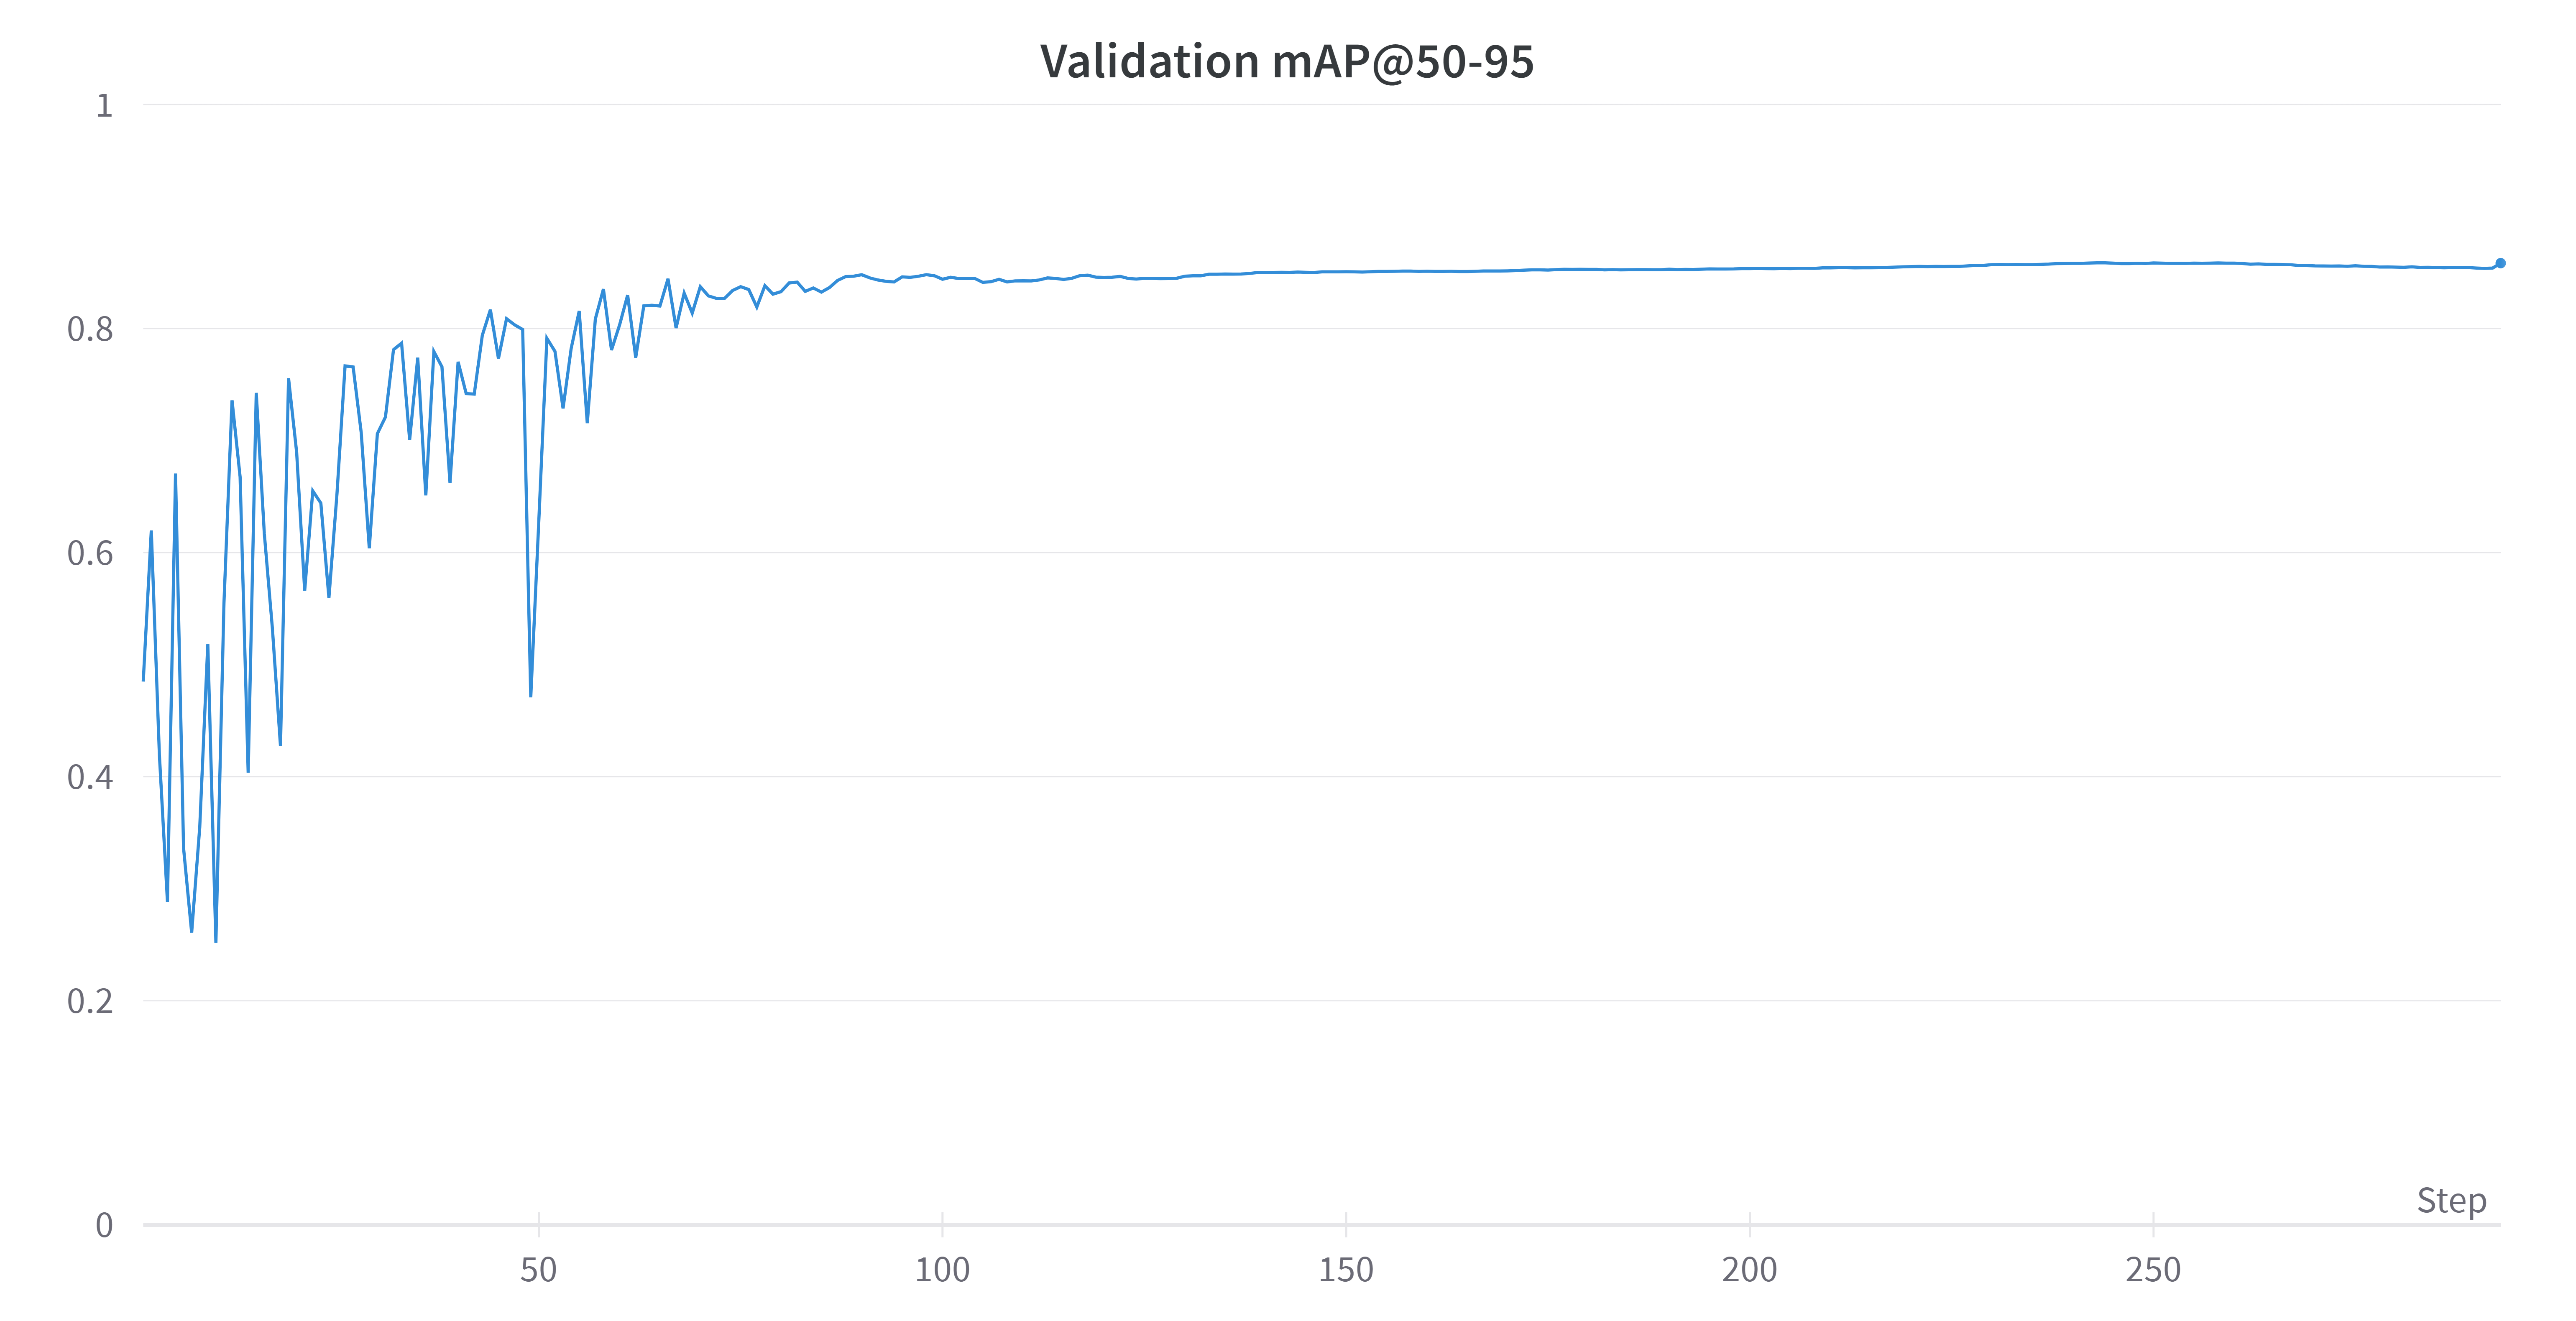
\includegraphics[width=\textwidth]{figures/06_results/mAP5095Detector.png}
		\caption{\footnotesize{Validation mAP@50-95 curves of YOLOv8 with the bigger and harder dataset.}}
		\label{fig:validation mAP50-95 Final}
	\end{subfigure}
	
	\caption[Validation mAP@50-95 curves of YOLOv8]{\footnotesize{Validation mAP@50-95 curves of YOLOv8 trained and validated with a dataset and a previous version of the same dataset.}}
	\label{fig:validation mAP50-95}
\end{figure}

{
    Figures \ref{fig:detector_precision}, \ref{fig:detector_recall} and \ref{fig:detector_f1score} present the precision, recall and F1-Score metrics, assessed at various confidence thresholds. 
    When transitioning from detection to tracking, the primary objective is to attain a high recall rate to minimize the loss of ants during the tracking phase. This approach is rooted in the rationale that spurious false positives can be subsequently filtered out by the tracking model.
}

{
	As seen on Figure \ref{fig:detector_f1score}, the optimal F1-Score on the validation set occurs at 0.5. 
    For the tracking model, the minimum detection confidence parameter was set to 0.4. 
    This choice deliberately shift towards a higher recall because the tracking process is able to filter spurious false positives out.
}

{
    Furthermore, the low-high confidence threshold was set at 0.8. 
    At this threshold, the impact of a reduced recall on the F1-Score becomes noticeable, prompting a thoughtful balance in model performance.
}

{
    The training of the \ac{YOLOv8n} model was performed on CALCULA, the computing server from the \ac{TSC} department of the \ac{UPC}, using 1 GPU NVIDIA GeForce RTX 3090 with 24 GB of memory available, 16 cores of CPU and 32 GB of RAM. With this setting and the previously explained hyperparameters (on Table \ref{tab:detection hyperparameters}), the longest training duration was smaller than 7 hours.
}

\begin{figure}[!p]
	\centering
	\begin{subfigure}[]{0.45\textwidth}
        \centering
		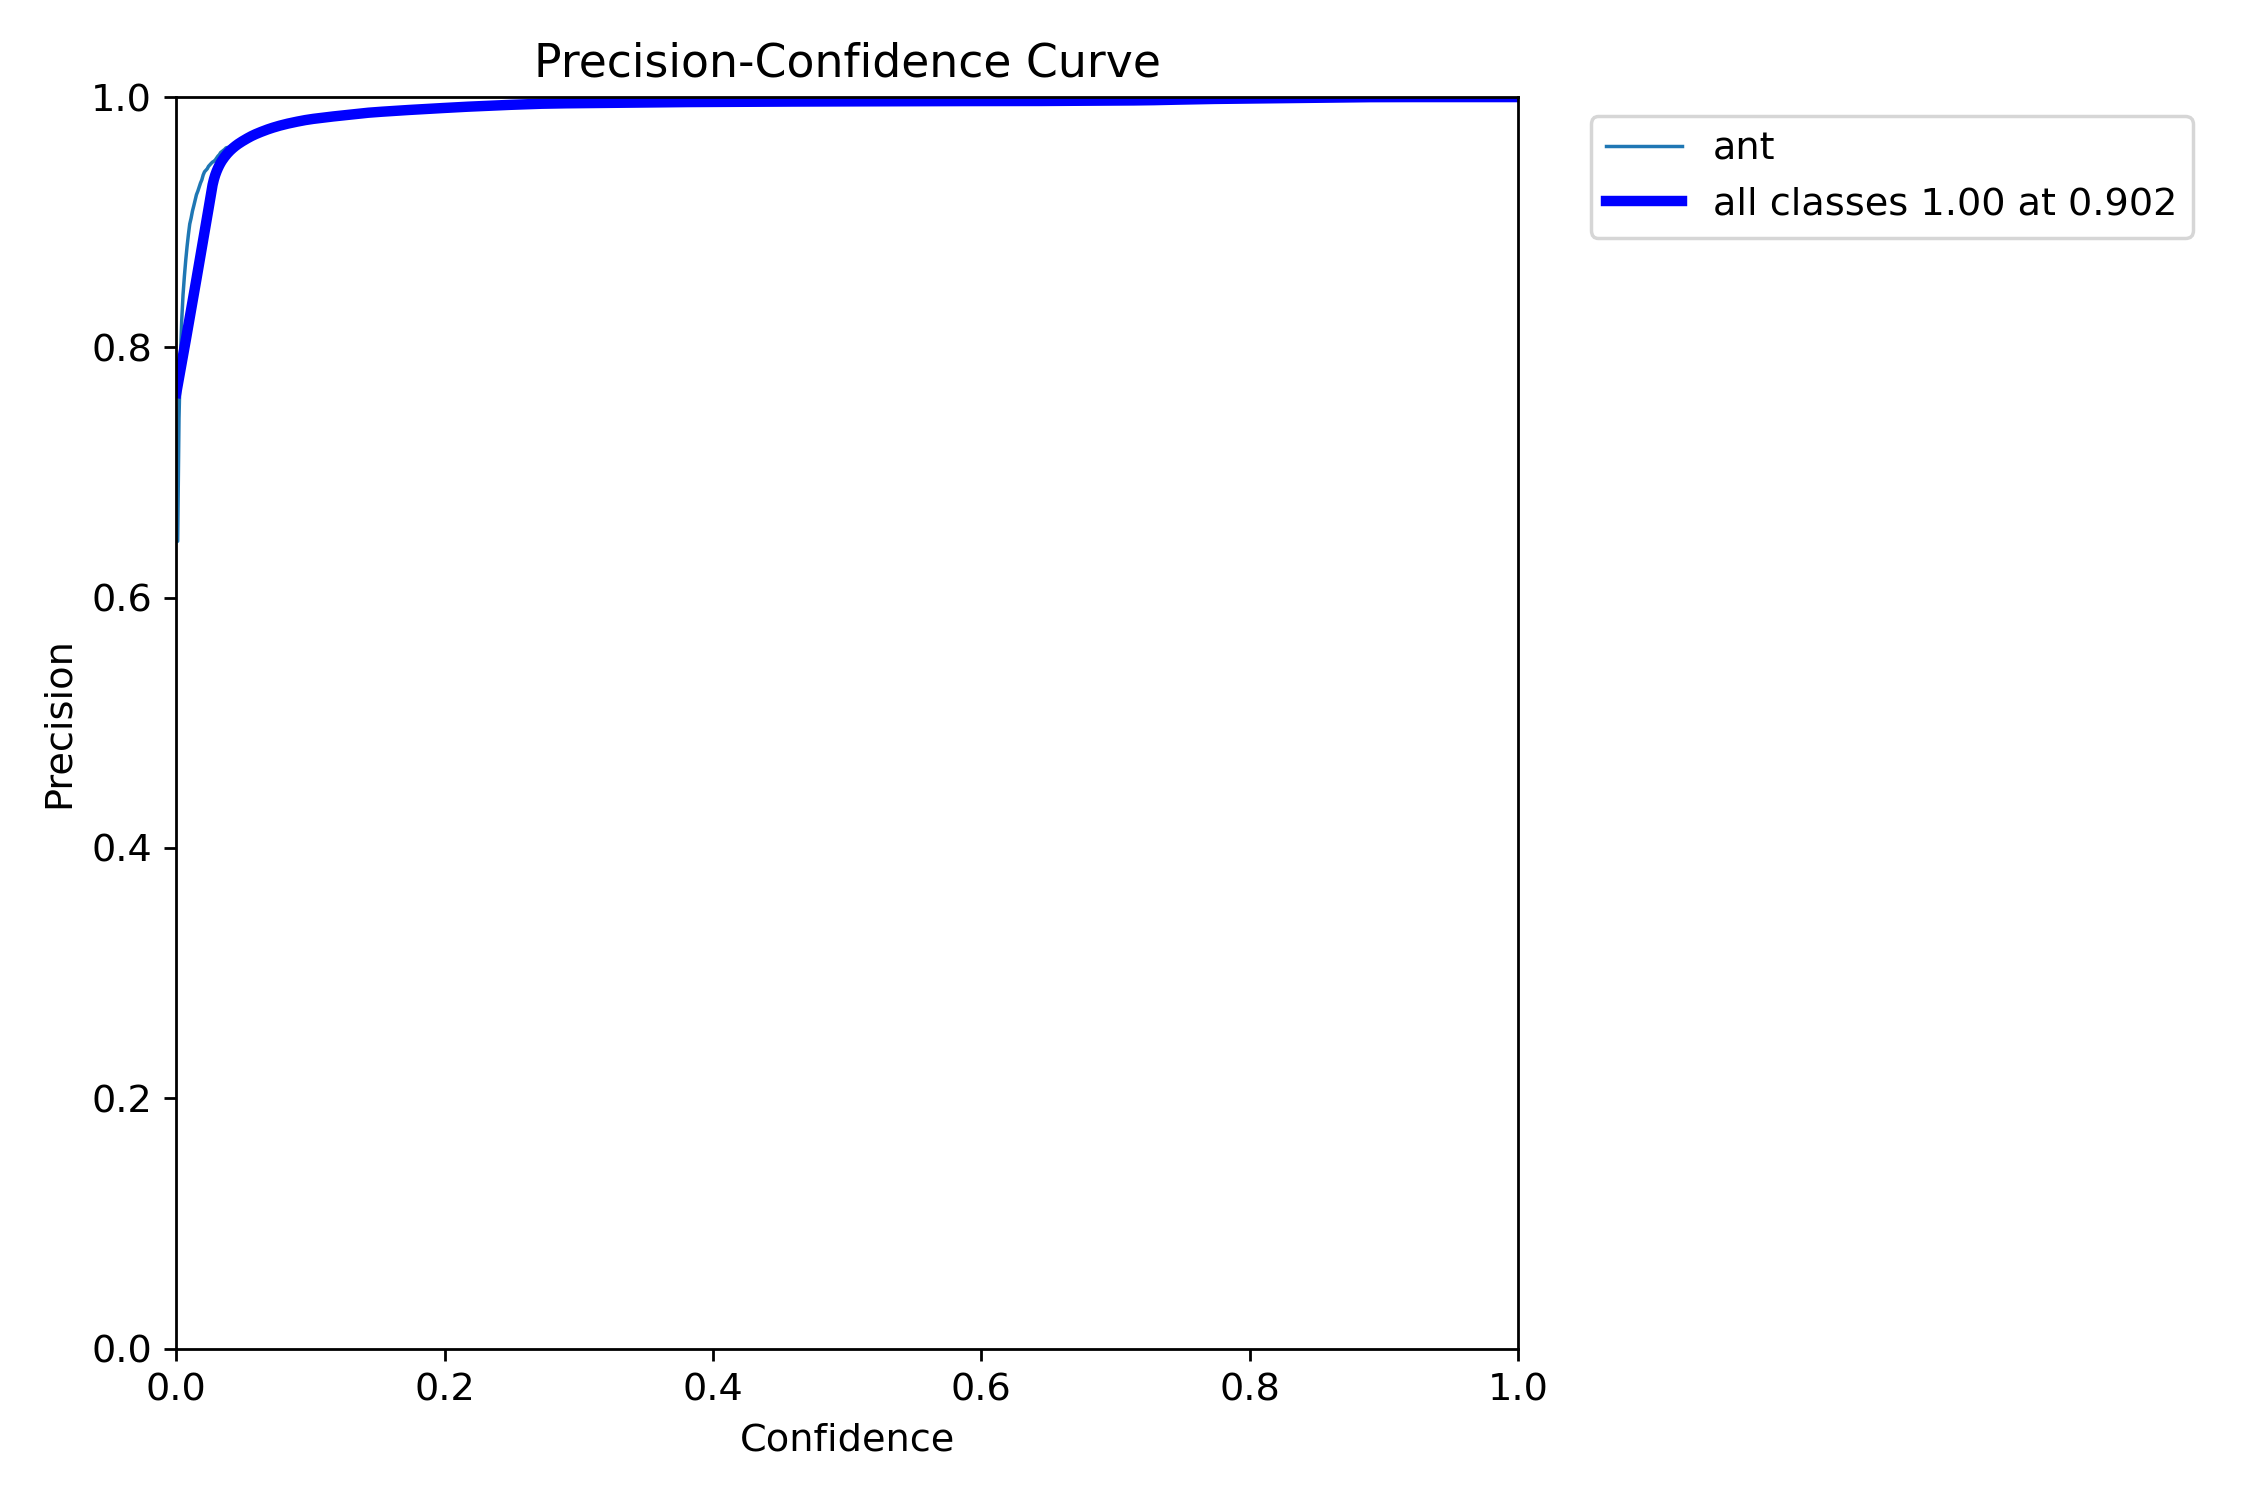
\includegraphics[width=\textwidth]{figures/06_results/PrecisionCurveDetector.png}
        \caption[Precision-Confidence curve of YOLOv8]{\footnotesize{Precision-Confidence curve.}}
        \label{fig:detector_precision}
	\end{subfigure}
	\begin{subfigure}[]{0.45\textwidth}
        \centering
		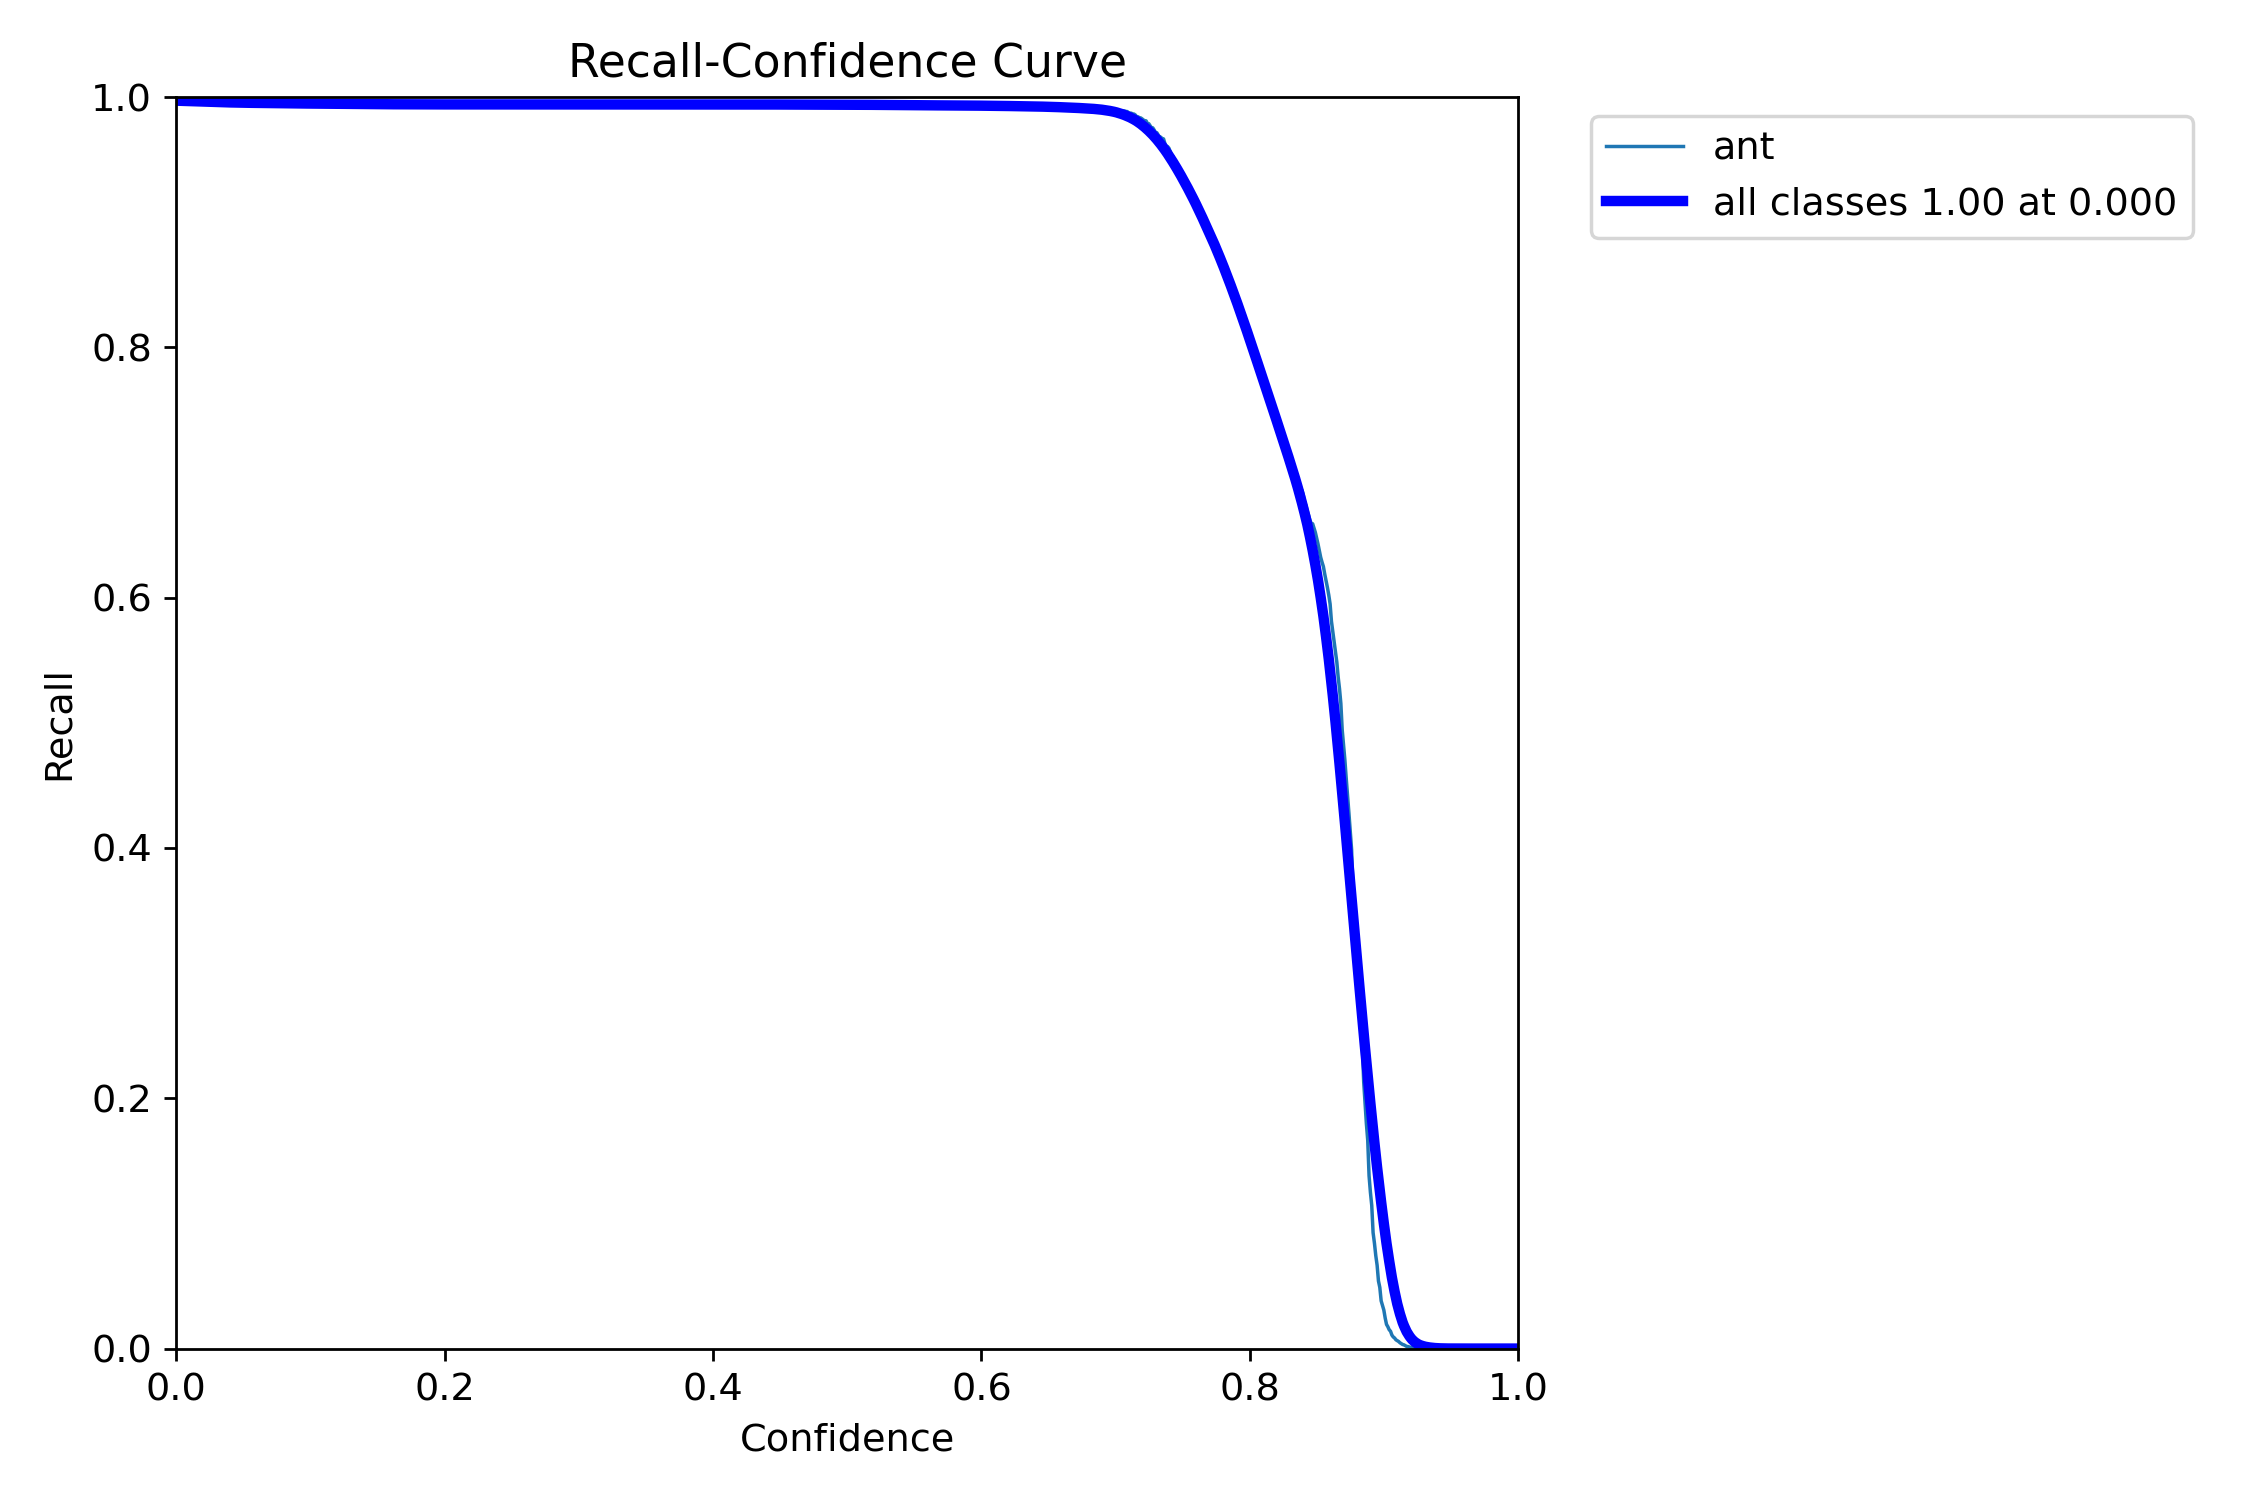
\includegraphics[width=\textwidth]{figures/06_results/RecallCurveDetector.png}
        \caption[Recall-Confidence curve of YOLOv8]{\footnotesize{Recall-Confidence curve.}}
        \label{fig:detector_recall}
	\end{subfigure}

    \begin{subfigure}[]{0.45\textwidth}
        \centering
		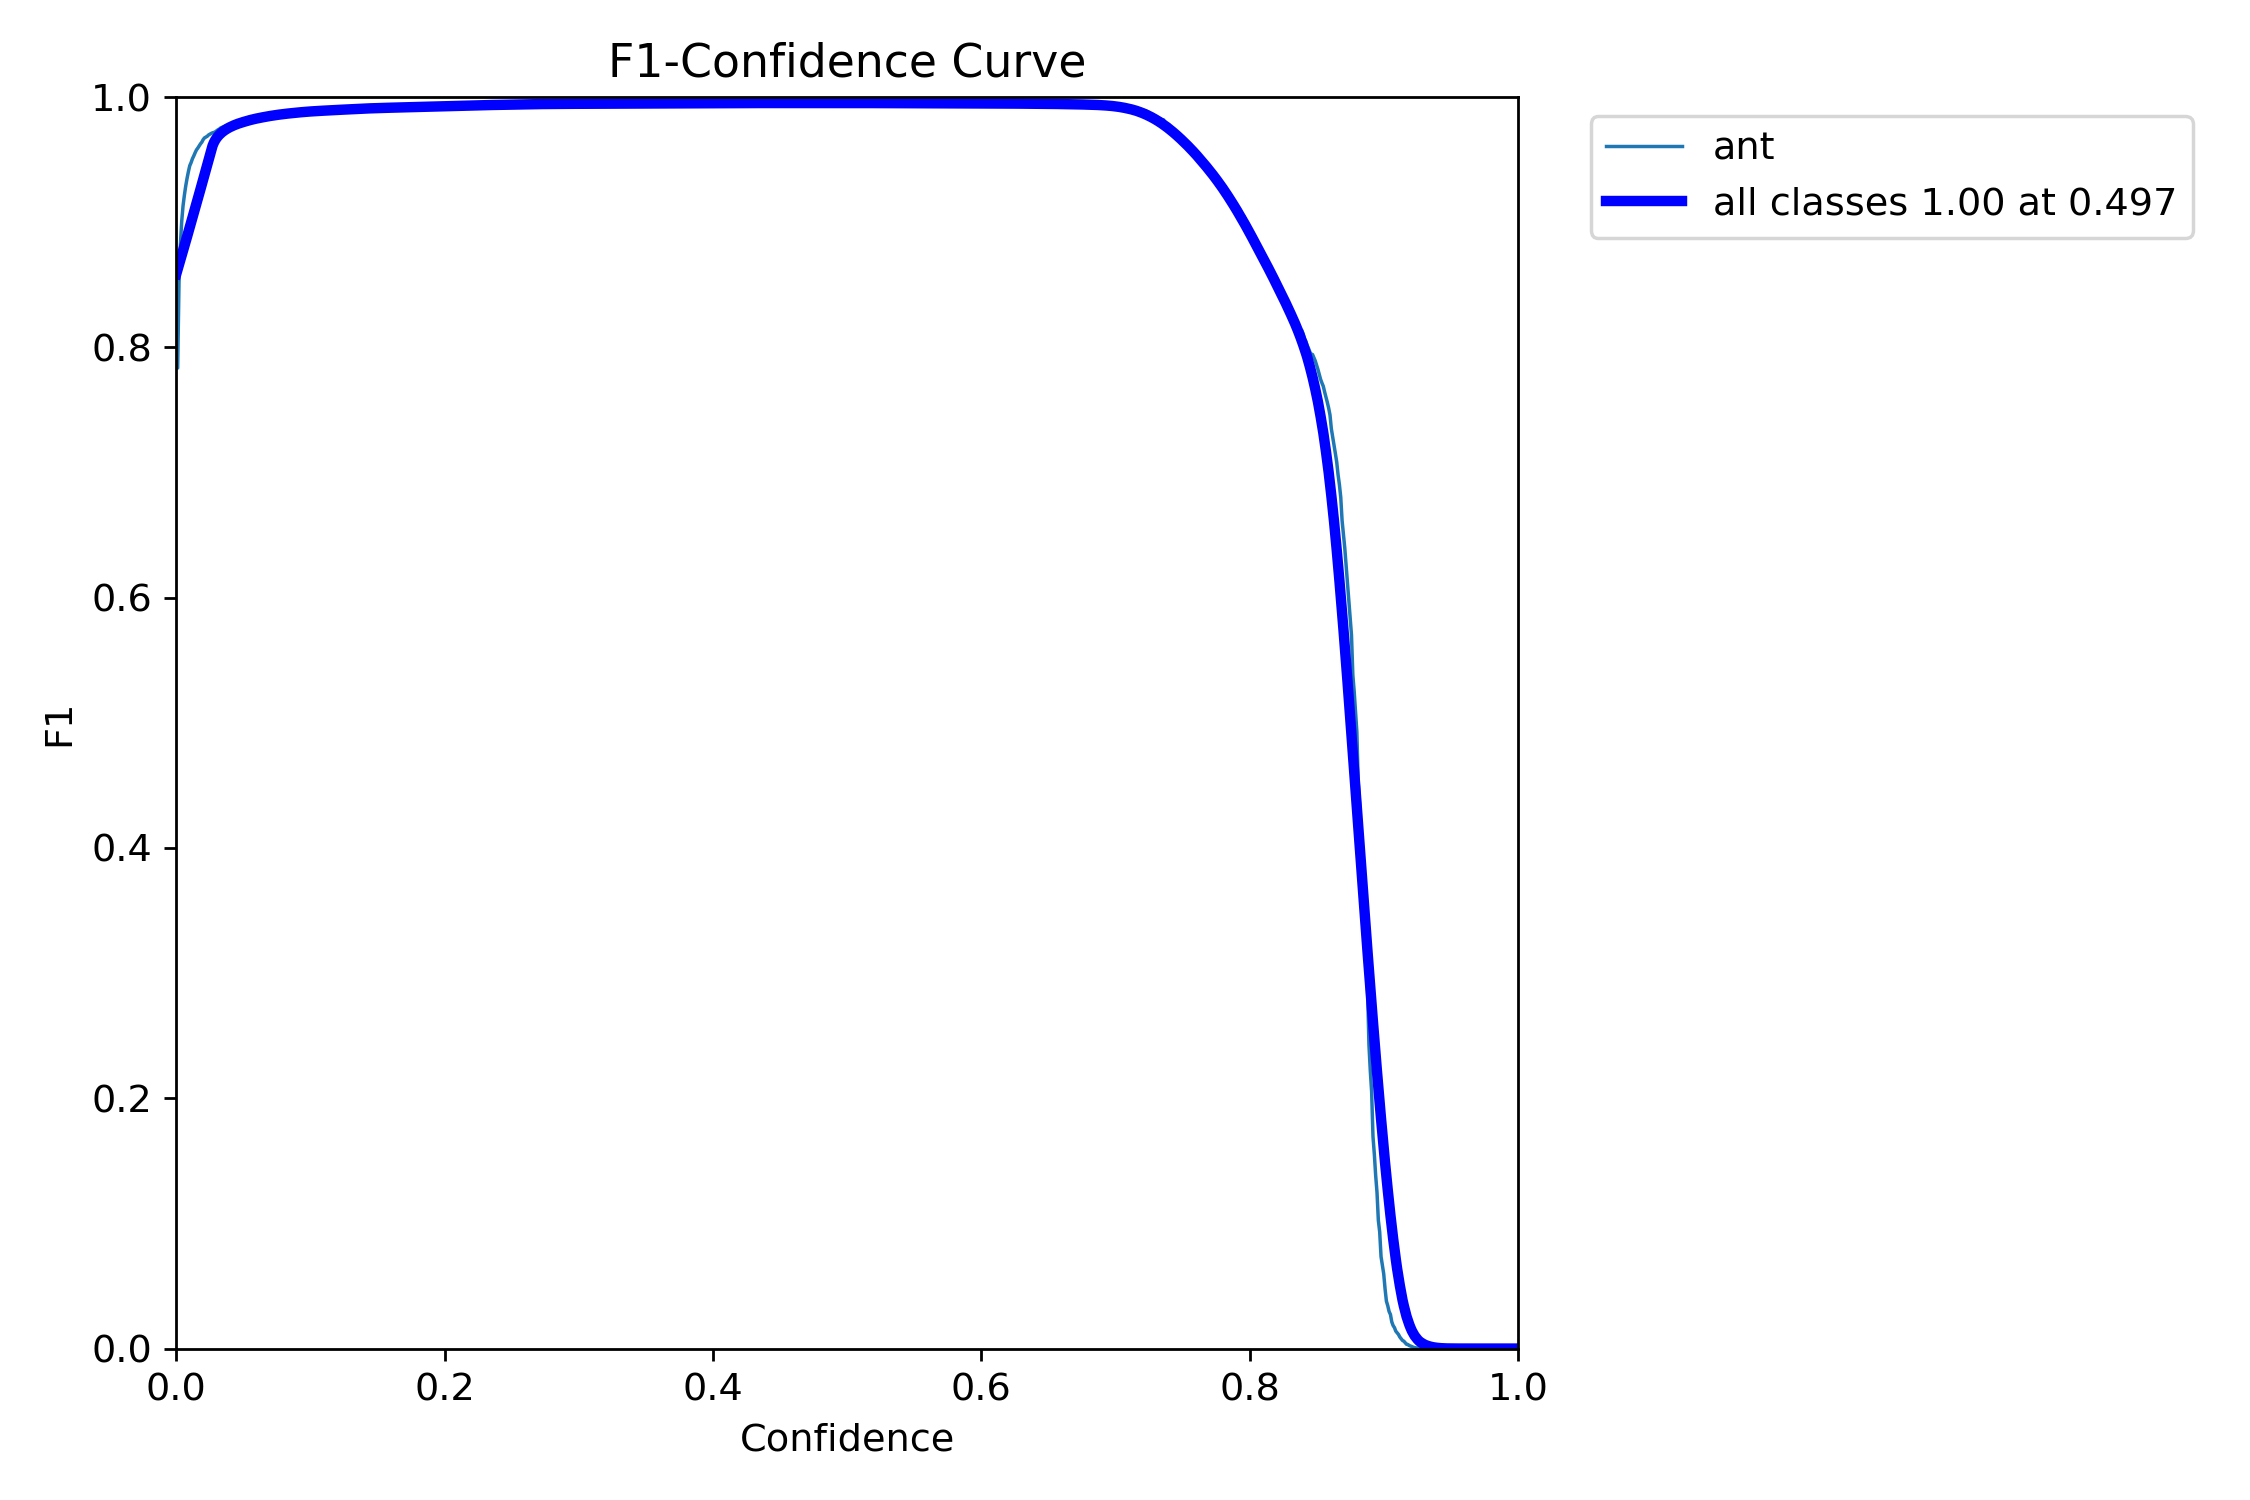
\includegraphics[width=\textwidth]{figures/06_results/F1_curveDetector.png}
        \caption[F1Score-Confidence curve of YOLOv8]{\footnotesize{F1Score-Confidence curve.}}
        \label{fig:detector_f1score}
	\end{subfigure}
	
	\caption[YOLOv8: Precision, Recall and F1Score-Confidence curve]{\footnotesize{Validation curves of the trained YOLOv8 for confidence thresholding.}}
	\label{fig:detector_precision_recall_f1}
\end{figure}

\FloatBarrier

\needspace{0.25\textheight}
\subsection{Detection Results}

{
    In object tracking, the selection of a detection model significantly impacts precise location estimation. 
    Table \ref{tab:detection-comparison} reinforces the rationale behind the chosen detection model by comparing its mean average precision, precision and recall with other trained models and the background extraction model. 
}

\begin{table}[H]
    \centering
    \caption[Detectors mAP Comparison]{ \footnotesize Comparison of detectors \ac{mAP} on the testing video when the minimum confidence threshold is 0.4.}
    \label{tab:detection-comparison}

    \begin{tabularx}{\textwidth}{
        @{\hspace{0.025\textwidth}}
        >{\raggedright\arraybackslash}X
        >{\centering\arraybackslash}p{0.175\textwidth}|
        >{\centering\arraybackslash}p{0.175\textwidth}|
        >{\centering\arraybackslash}p{0.175\textwidth}|
        >{\centering\arraybackslash}p{0.175\textwidth}
        @{\hspace{0.025\textwidth}}
    }
        \toprule
        \textbf{Model Name} & \textbf{mAP@50} & \textbf{mAP@50-95} & \textbf{Precision} & \textbf{Recall} \\
        \midrule
        \midrule
        Background extraction & 21\% & 8\% & 46\% & 28\% \\
        YOLOv8n & 30\% & 15\% & 48\% & 44\% \\
        \bottomrule
    \end{tabularx}
\end{table}

{
    The data unequivocally demonstrates the superiority of YOLOv8n over the background extraction baseline across all evaluated aspects. 
    Particularly noteworthy is the substantial improvement in recall. 
}

{
    However, comparing the metrics on this testing set with the perfect results in the validation set depicted in Figure \ref{fig:detector_precision_recall_f1}, 
    it can be seen that the model's ability to generalize or the dissimilarity of the test set compared to the training and the validation sets should be considered. 
    Further improvements may be possible with a larger dataset.
}


\needspace{0.25\textheight}
\subsection{Appearance Training}



{
    The appearance model is a key component for trackers based on re-identification. 
    However, unlike the stable training curves from the detector, the appearance model metrics and loss curves resulted in swift overfitting (see Figures \ref{fig:training appearance}, \ref{fig:appearance mAP50} and \ref{fig:appearanceRank1}).
}

{
    The depicted curves on the Figures \ref{fig:training appearance}, \ref{fig:appearance mAP50} and \ref{fig:appearanceRank1} represent the best two trained models, 
	one reached the best score and the other was the nearest scores without a clear drop in the validation metric (best training). 
	In both cases, an early stop strategy was applied (the best score model keep the weights of the epoch 5500 and the best training keep the weights of the epoch 33000).
}

{
	The curves reveal a rapid convergence on the training data, as depicted in Figure \ref{fig:training appearance}. 
	However, a notable trend of stagnation or decline becomes evident in the validation results, as illustrated in Figures \ref{fig:appearance mAP50} and \ref{fig:appearanceRank1}. 
	The decline in the validation metric, along with the improvement in the loss, is indicative of overfitting.
	A closer examination of the learning rates reveals that the best training model, characterized by its absence of decline, operates with a higher learning rate. 
	Since the training convergence can be attributed to the dataset's relative simplicity in terms of data quantity, 
	both training processes can be categorized as overfitted, and the elevated learning rate might have prevented a more severe overfitting compared to the best score model.
}

{
    While the model seems to yields features that contains ant individualities, with a rank-1 accuracy of 74\%, 
	it is difficult to measure its performance from the training and validation curves alone.
}

{
    The presented training results are only from the unoriented dataset; the oriented dataset (containing the same data) yielded a worse rank-1 accuracy with the same issues on the training.
}

\needspace{0.1\textheight}

{
    The training of the \ac{BoT} model was performed on CALCULA using 4 GPUs NVIDIA GeForce GTX 1080 Ti, 8 cores of CPU and 128 GB of RAM (because the code had some memory leakage due to multiprocessing and data stored on non-consecutive memory). With this setting and the previous hyperparameters, the longest training duration was smaller than 1 hour.
}

%\vspace{-1em}

\begin{figure}[!h]
	\centering
	\begin{subfigure}[]{0.9\textwidth}
		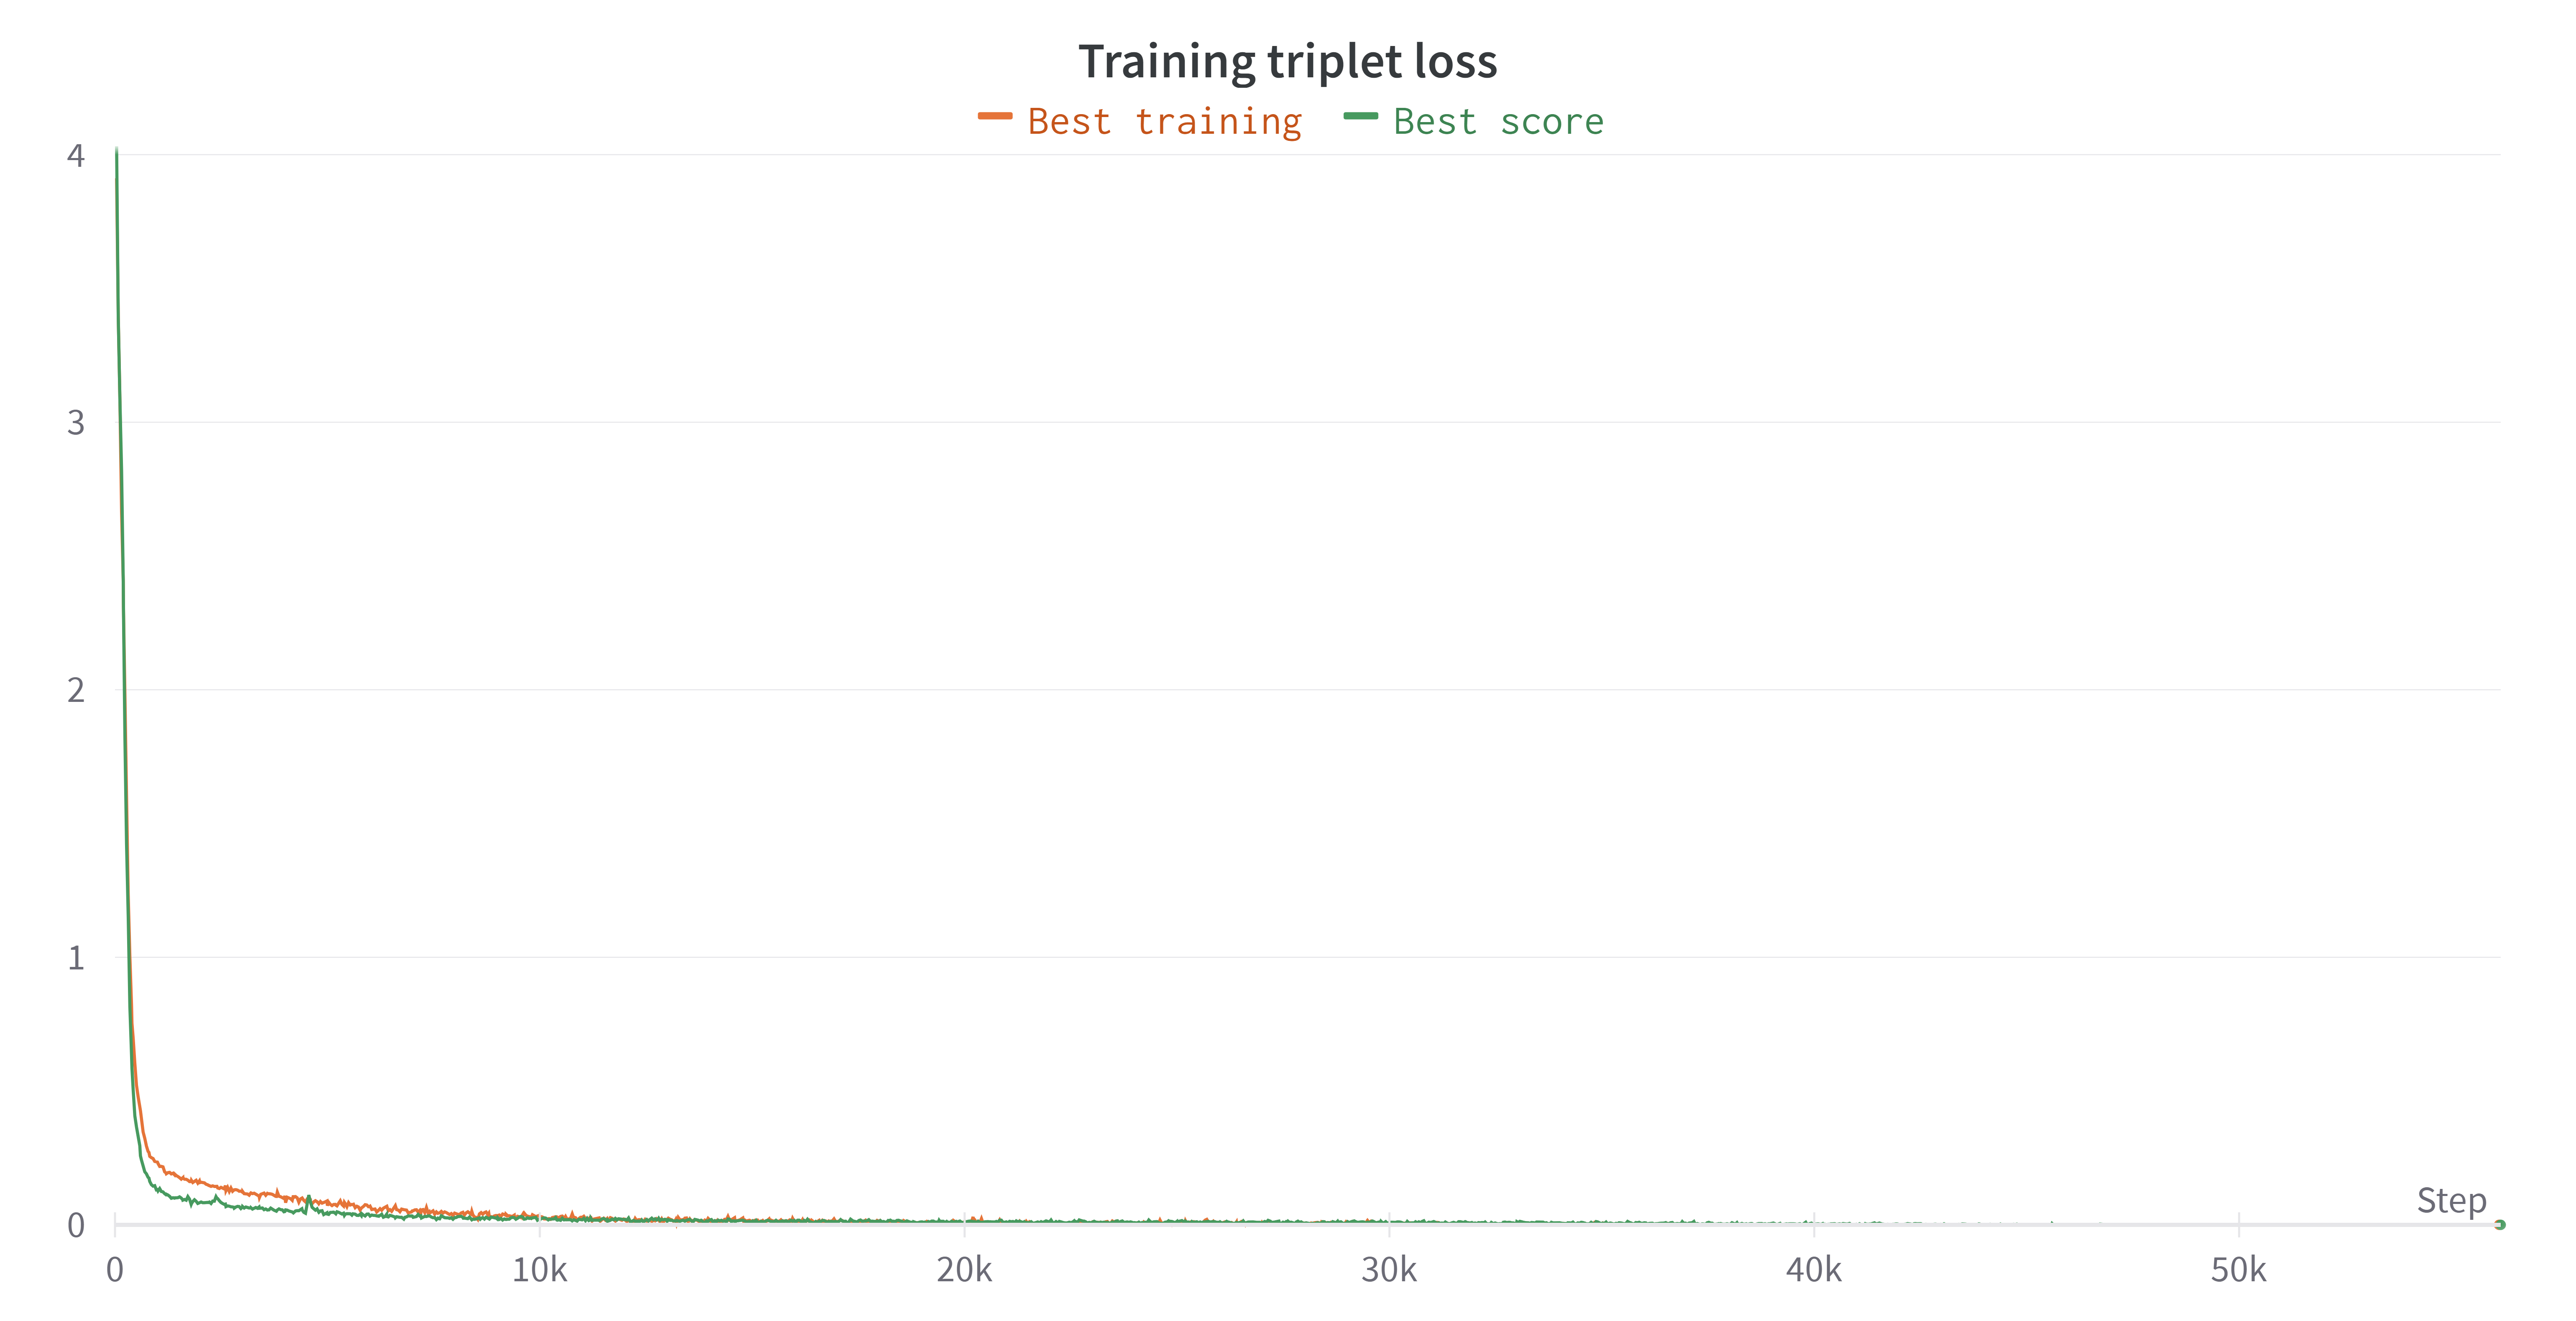
\includegraphics[width=\textwidth]{figures/06_results/ApperanceTrainTriplet.png}
		\caption{\footnotesize{Training triplet loss curve of BoT for two training settings.}}
		\label{fig:appearanceClass}
	\end{subfigure}
	\begin{subfigure}[]{0.9\textwidth}
		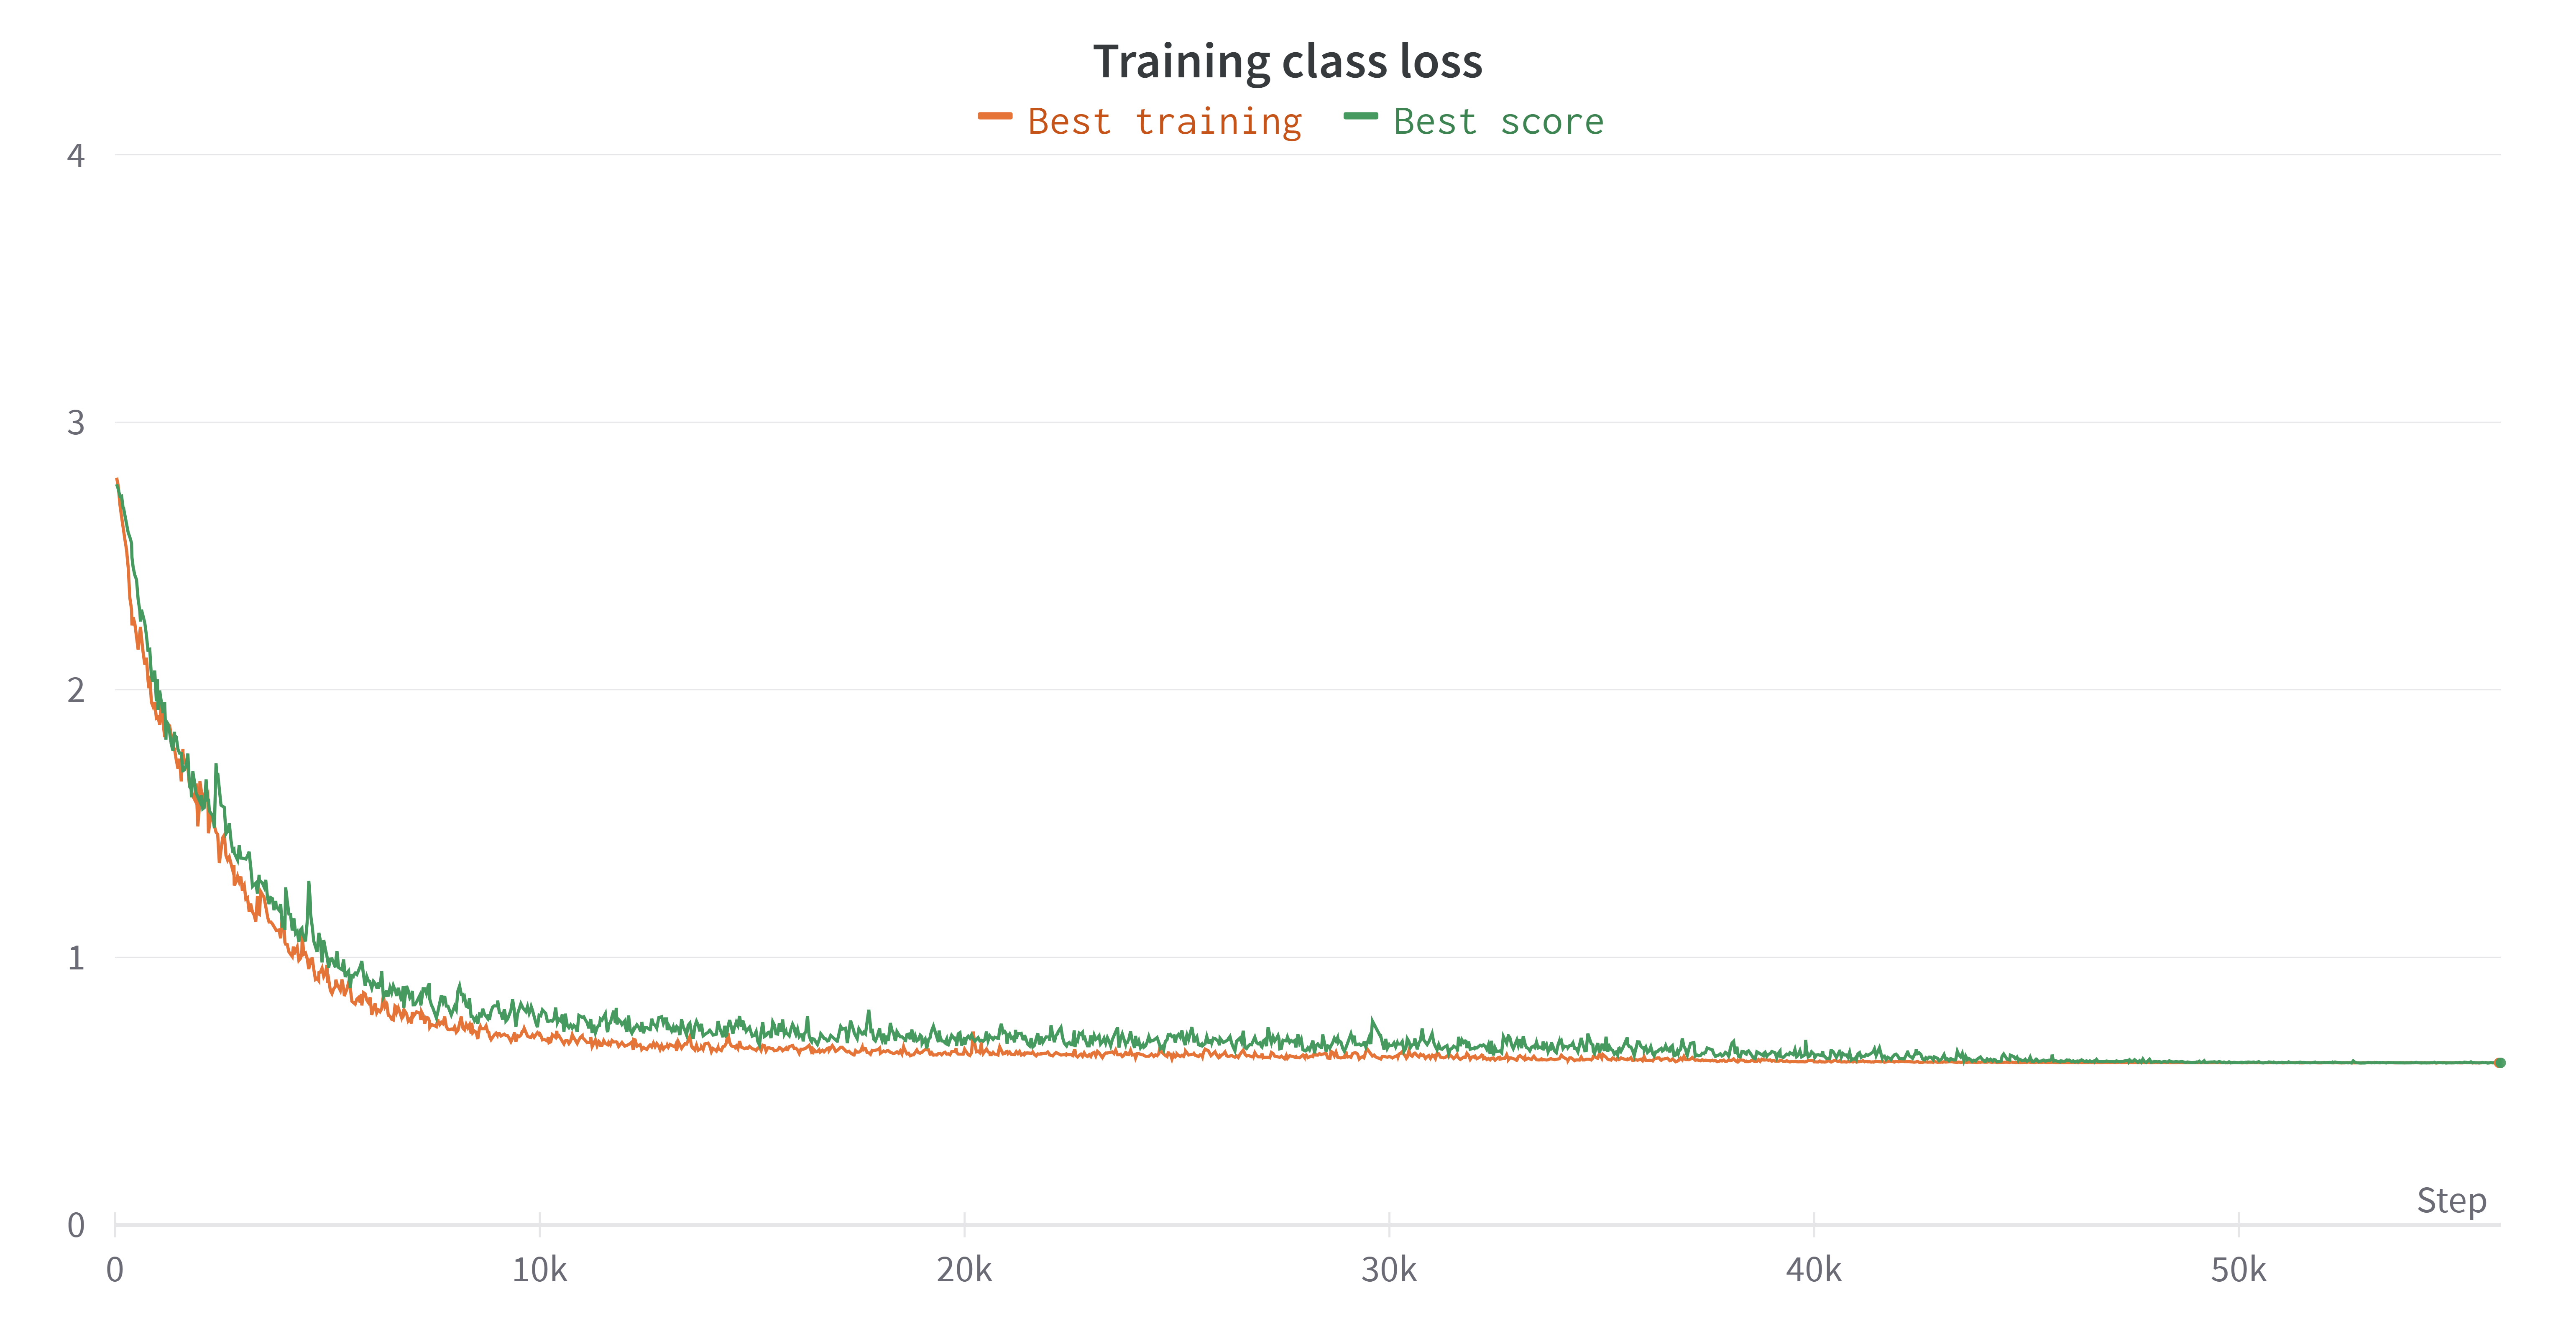
\includegraphics[width=\textwidth]{figures/06_results/ApperanceTrainClass.png}
		\caption{\footnotesize{Training classificationloss curve of BoT for two training settings.}}
		\label{fig:appearanceTriplet}
	\end{subfigure}
	
	\caption[Training Loss curves of BoT]{\footnotesize{Training Loss curves of BoT, it includes 2 training configurations.}}
	\label{fig:training appearance}
	\vspace{-4em}
\end{figure}

\begin{figure}[!p]
    \centering
    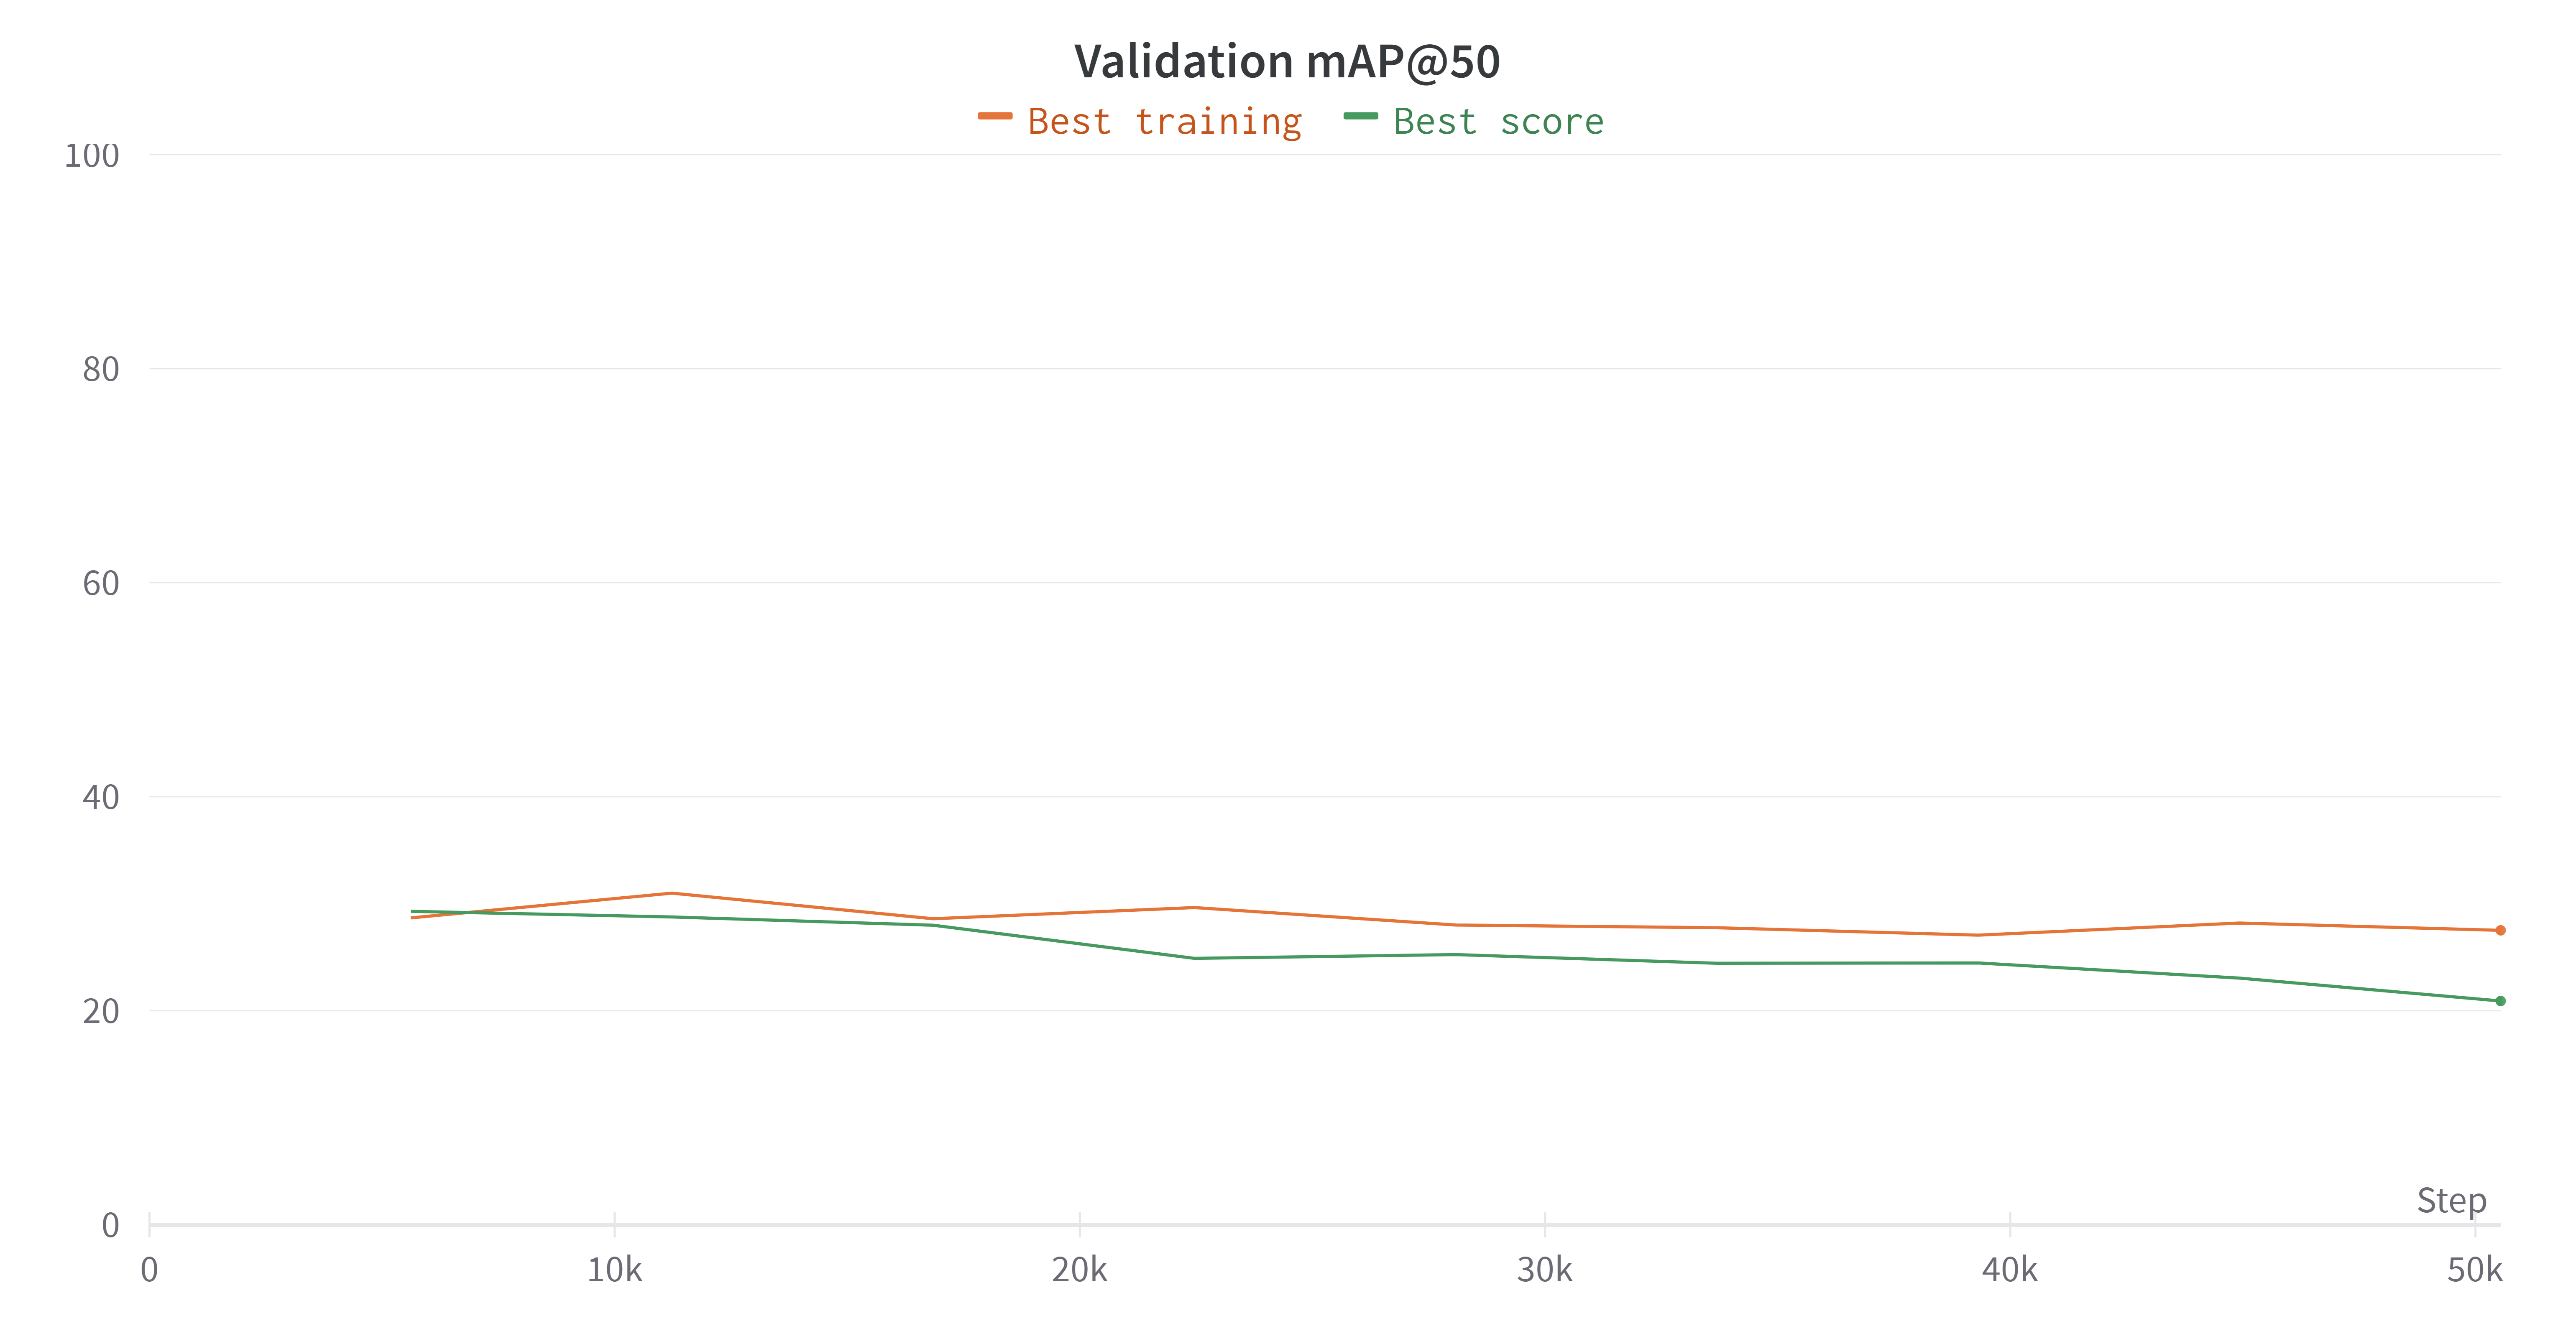
\includegraphics[width=0.9\textwidth]{figures/06_results/ApperanceValidationMAP.png}
    \caption[Validation mAP@50 curves of BoT]{\footnotesize{Validation mAP@50 curves of BoT for two training settings.}}
    \label{fig:appearance mAP50}
\end{figure}

\begin{figure}[!p]
	\centering
	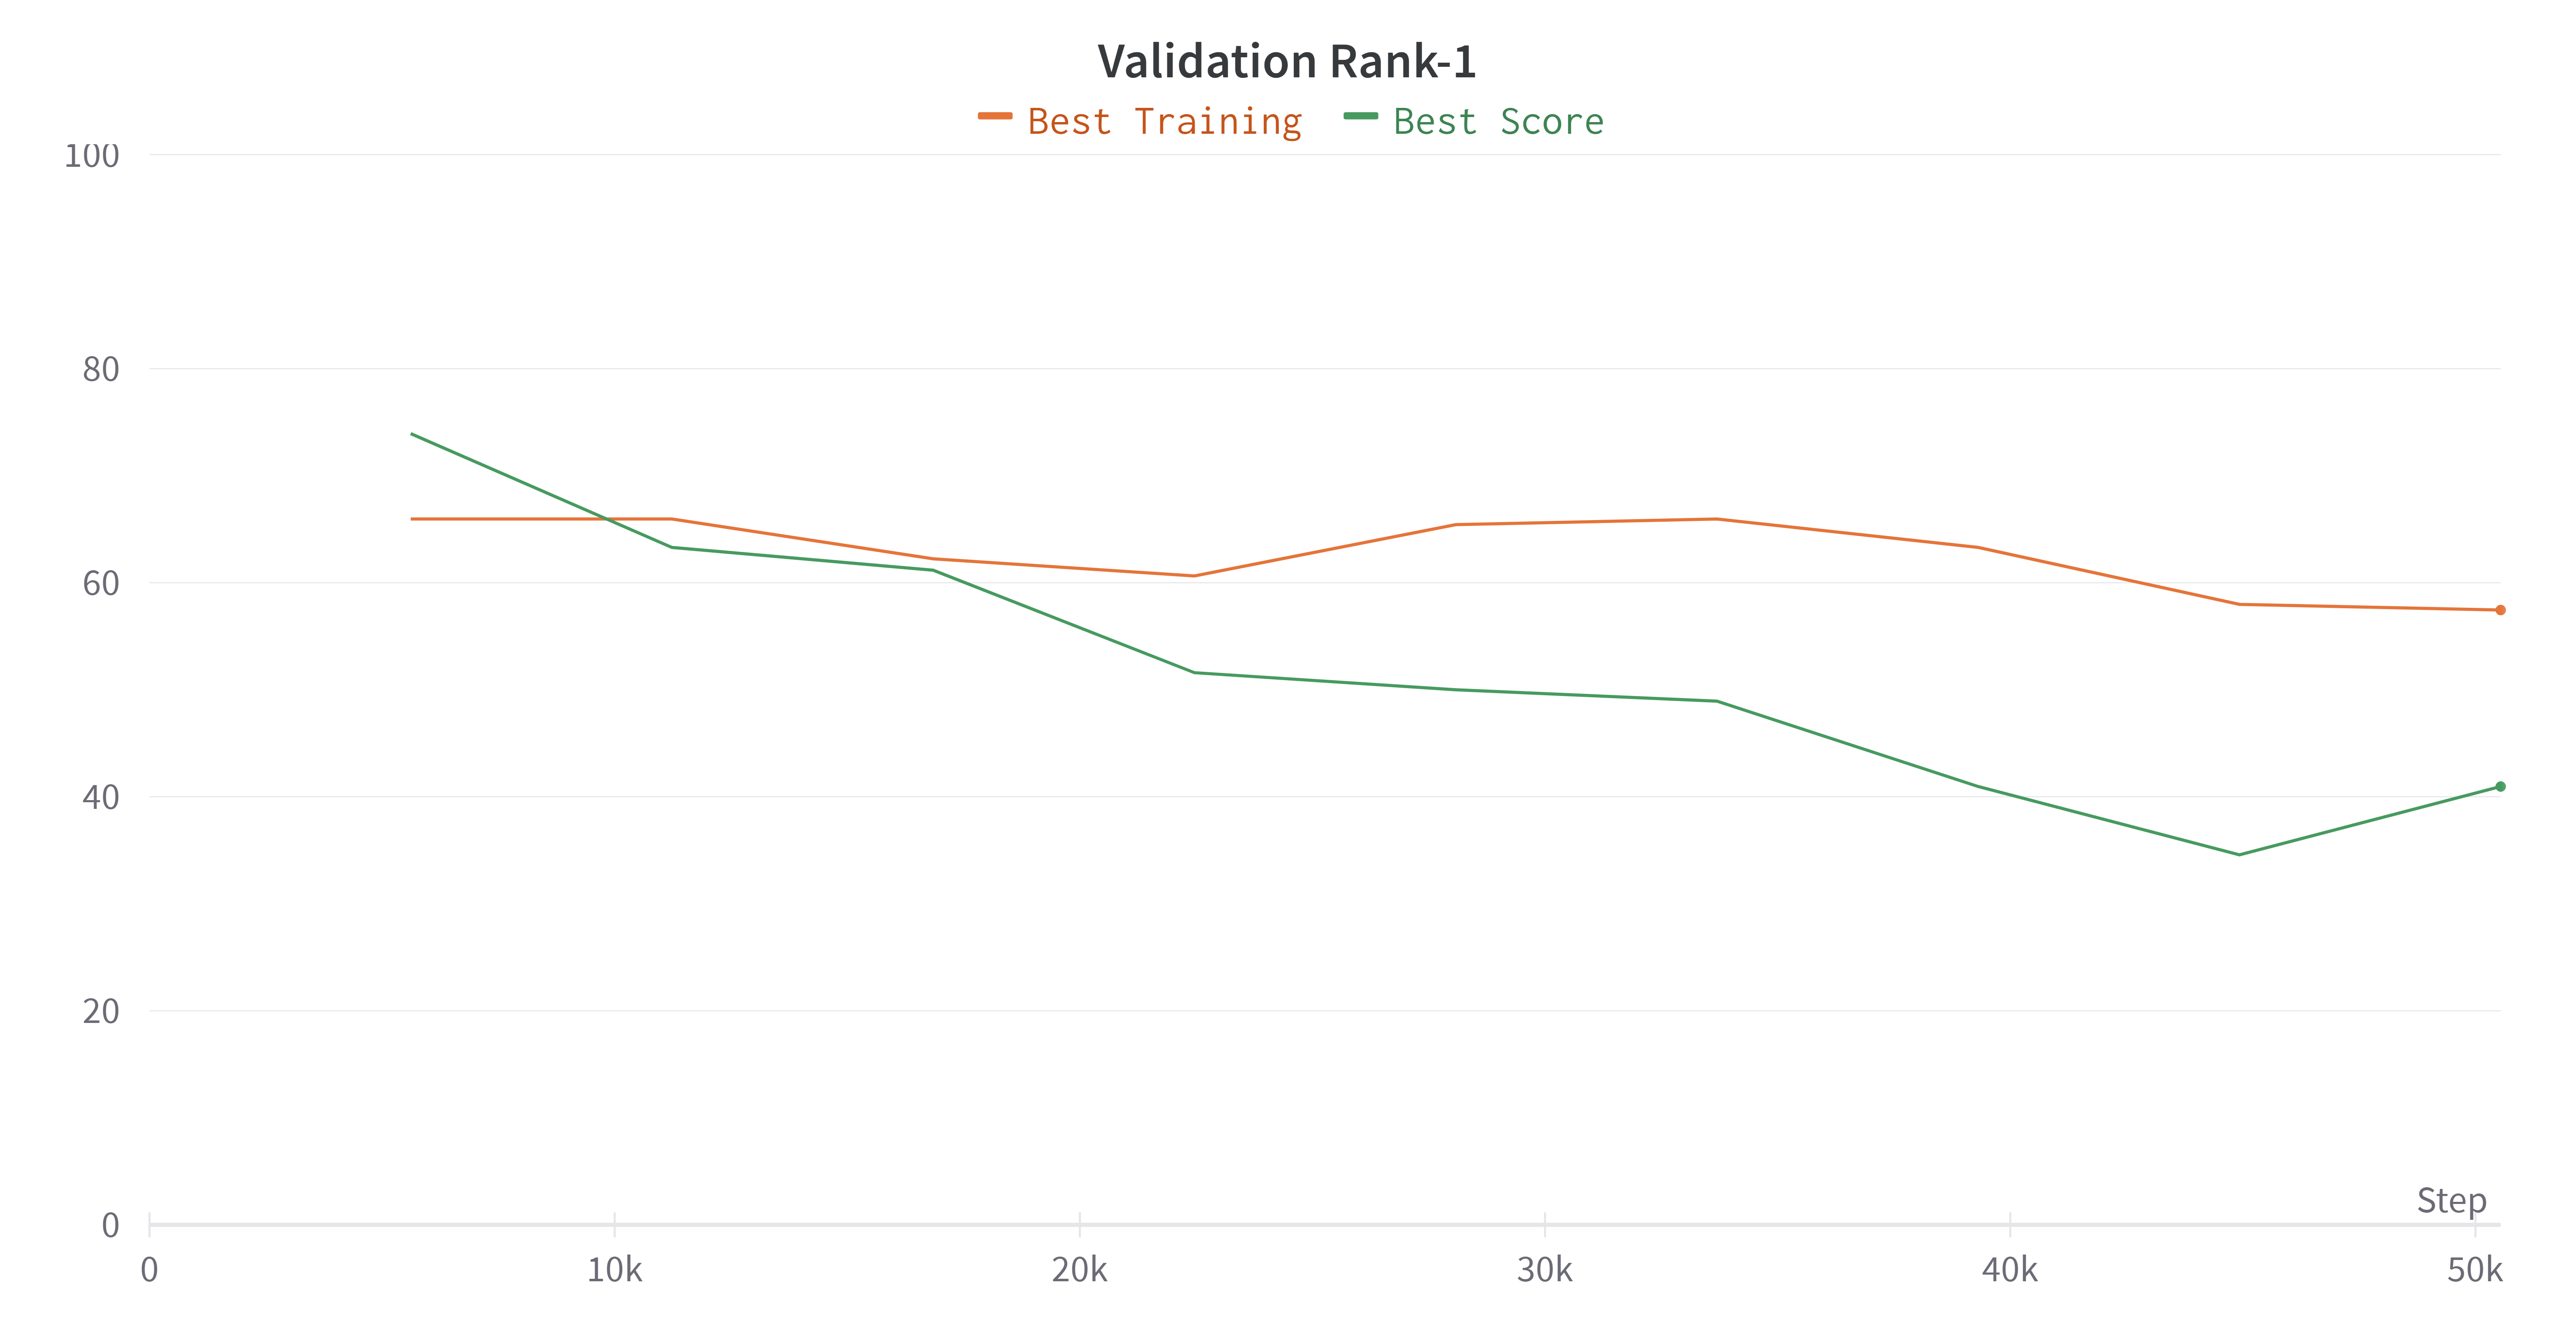
\includegraphics[width=0.9\textwidth]{figures/06_results/ApperanceValidationRank-1.png}
	\caption[Validation Rank-1 curve of BoT]{\footnotesize{Validation Rank-1 curve curve of BoT for two training settings.}}
	\label{fig:appearanceRank1}
\end{figure}

\FloatBarrier

\needspace{0.25\textheight}
\subsection{Appearance Tests Results} % 


{
    Figure \ref{fig:rotation_test} is the outcome of the rotation test where some ants representatives from the test ground truth are rotated and compared with the original detection and a random detection from another identity. 
    It consist in two polar plots with a characterization of the cosine distance applied on the appearance descriptors. 
}

{
    The left plot, when one crop of one ant is compared with itself, serves to demonstrate the non-invariability over rotation. 
    Without taking into account the 0º rotation with the expected distance 0, the distance is clearly higher at \textpm90º of rotation. 
    However, the fact that a 180º rotation contains another minimum suggests a future research direction: the usage of a body alignment algorithms in inference that allow solutions with a 180º rotation.
}

\begin{figure}[!hp]
    \centering
    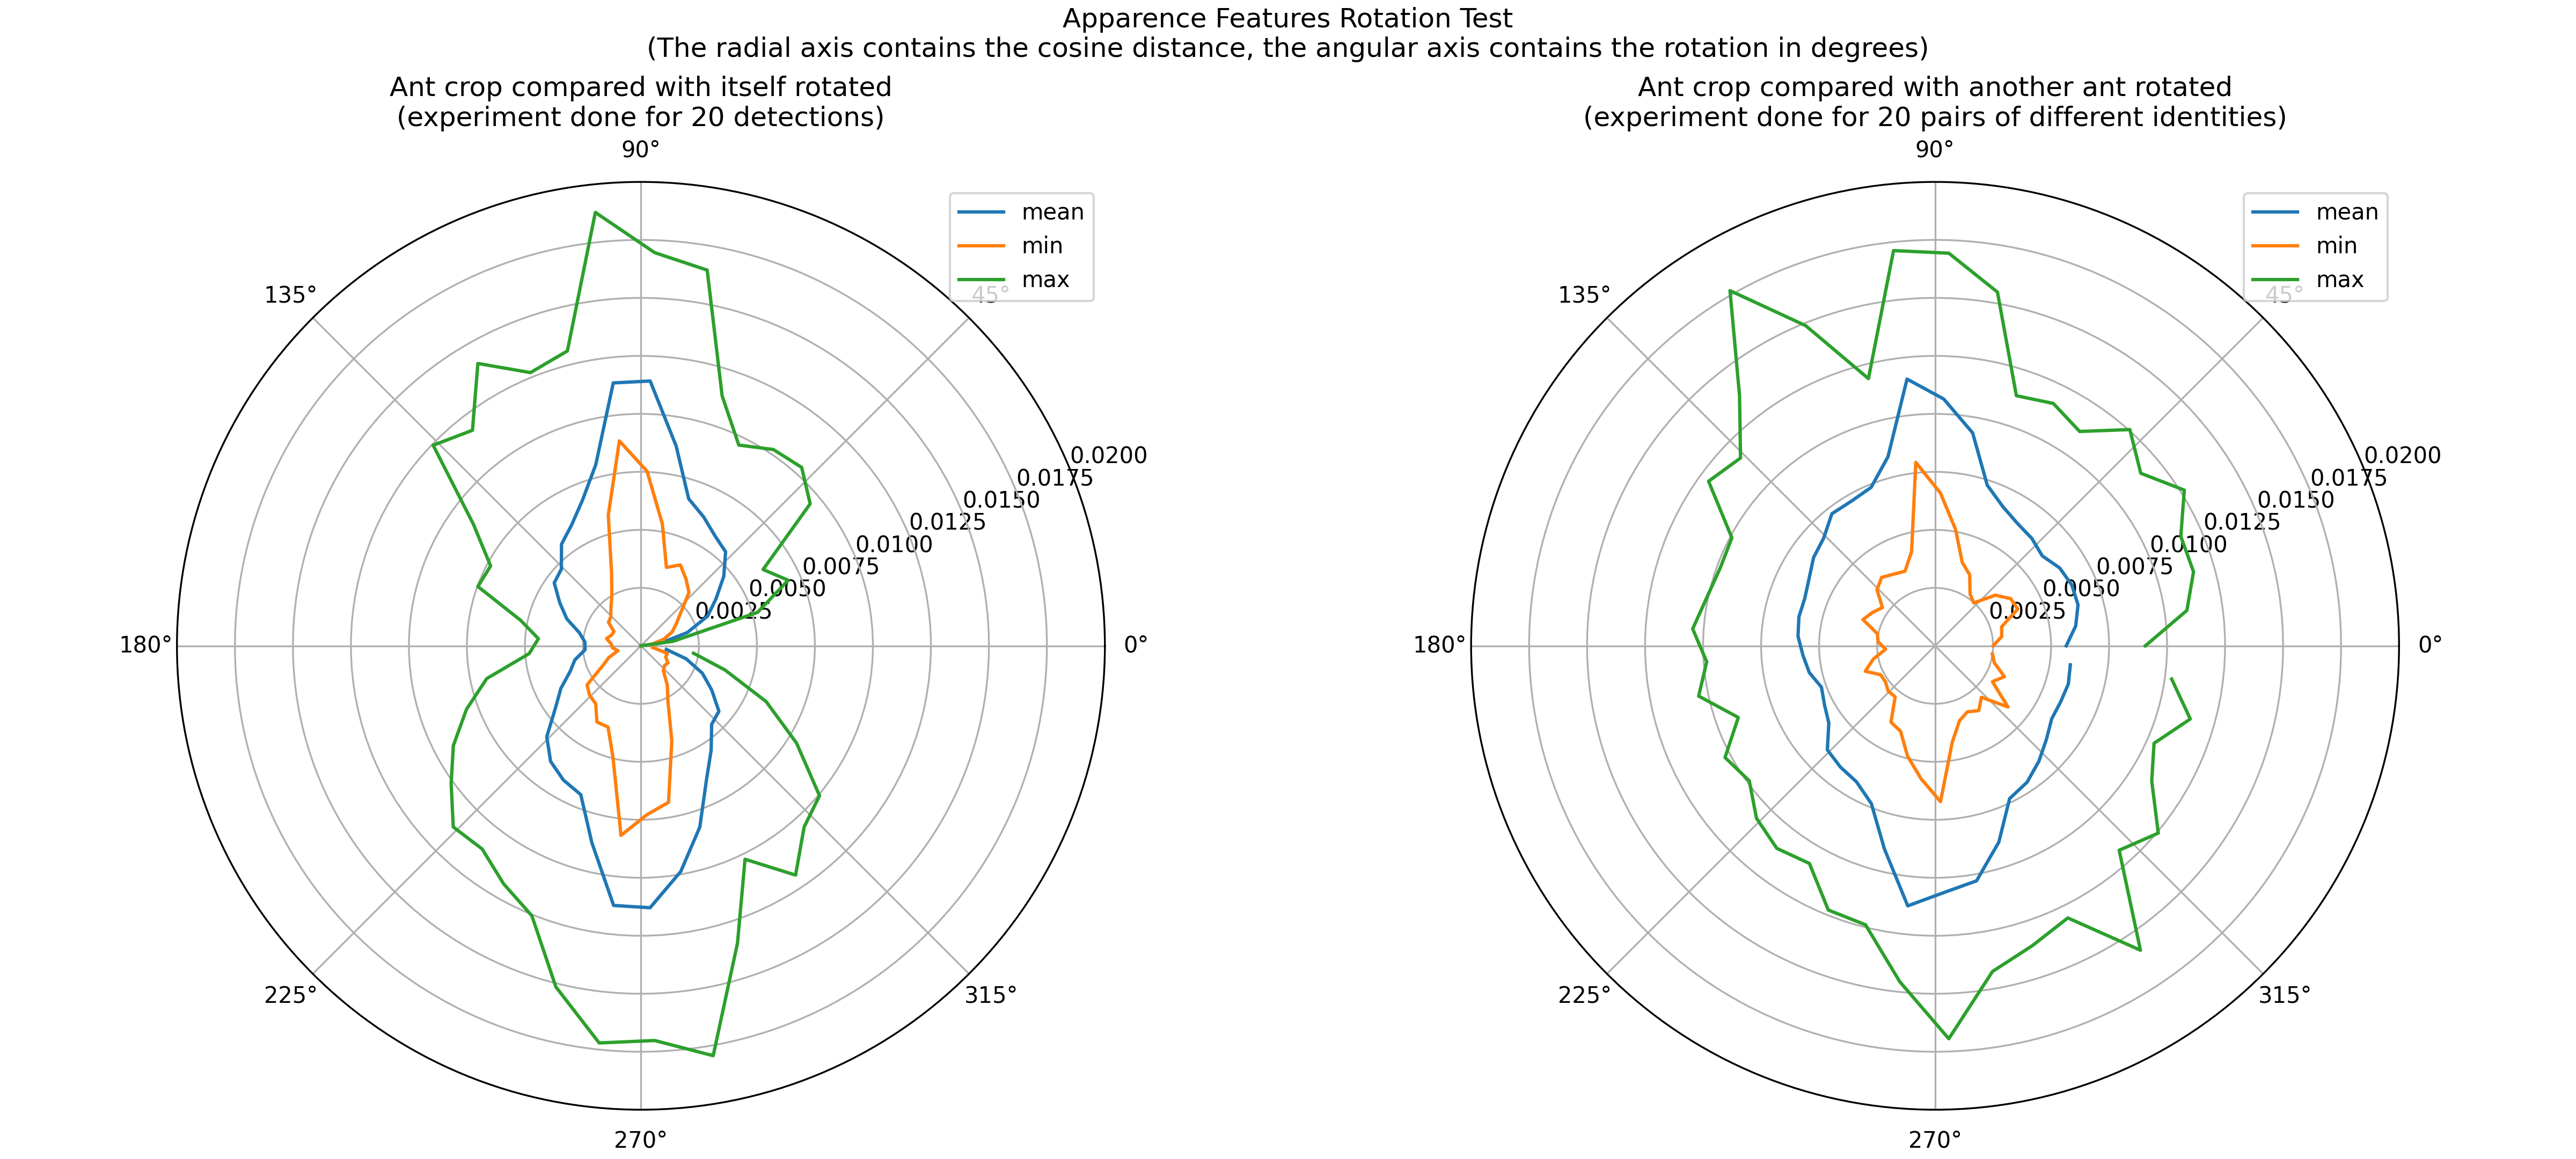
\includegraphics[width=0.8\textwidth]{figures/06_results/atr/rotation_all_ants_0-007.png}
    \caption[Appearance features rotation test]{\footnotesize{Validation of the rotation invariability property of the trained appearance features.}}
    \label{fig:rotation_test}
    \vspace{-1.5em}
\end{figure}

{
    The right plot of Figure \ref{fig:rotation_test}, when compared with the left plot, may provide an idea of the associability between tracks. 
    A 90º rotation makes one image as distant from itself as to another one. 
    However, to gain a clearer understanding, using the right plot to complement Figures \ref{fig:appearance_joinability} yields a clearer explanation.
}

{
    Figure \ref{fig:appearance_joinability_scope} depics the likelihood of correctly associating points where appearance is the most important feature: 
    the frames where ants are near each other. 
    When Figure \ref{fig:rotation_test} is examined, the tail of the probability density function for incorrect matches in Figure \ref{fig:appearance_joinability_scope} mainly contains distances related to a near 90º rotation of an ant with itself. 
}

{
    Figure \ref{fig:occlusion_scope} provides the ant displacement and duration of the instances where some ant is near another one.
    Most of these instances are short meetings within a small spatial scope, 
    this means that the most usual case is a small angular displacement because the ant did not have the time to rotate, 
    the better cases depicted in Figure \ref{fig:rotation_test}.
}

{
    Figure \ref{fig:appearance_joinability_all} exposes the distribution of means of distances for split tracklets within a single track and their comparison with tracklets from other tracks. 
    It is remarkable that the distributions are normalized in total area; in a real scenario, the problem tends to be unbalanced, with more negative cases than positives.   
}

\enlargethispage{1\baselineskip}

{
    It can be concluded that the appearance features are not usable yet, however, further research in this topic will still be relevant.
}

\begin{figure}[!hp]
	\centering
	\begin{subfigure}[]{0.49\textwidth}
		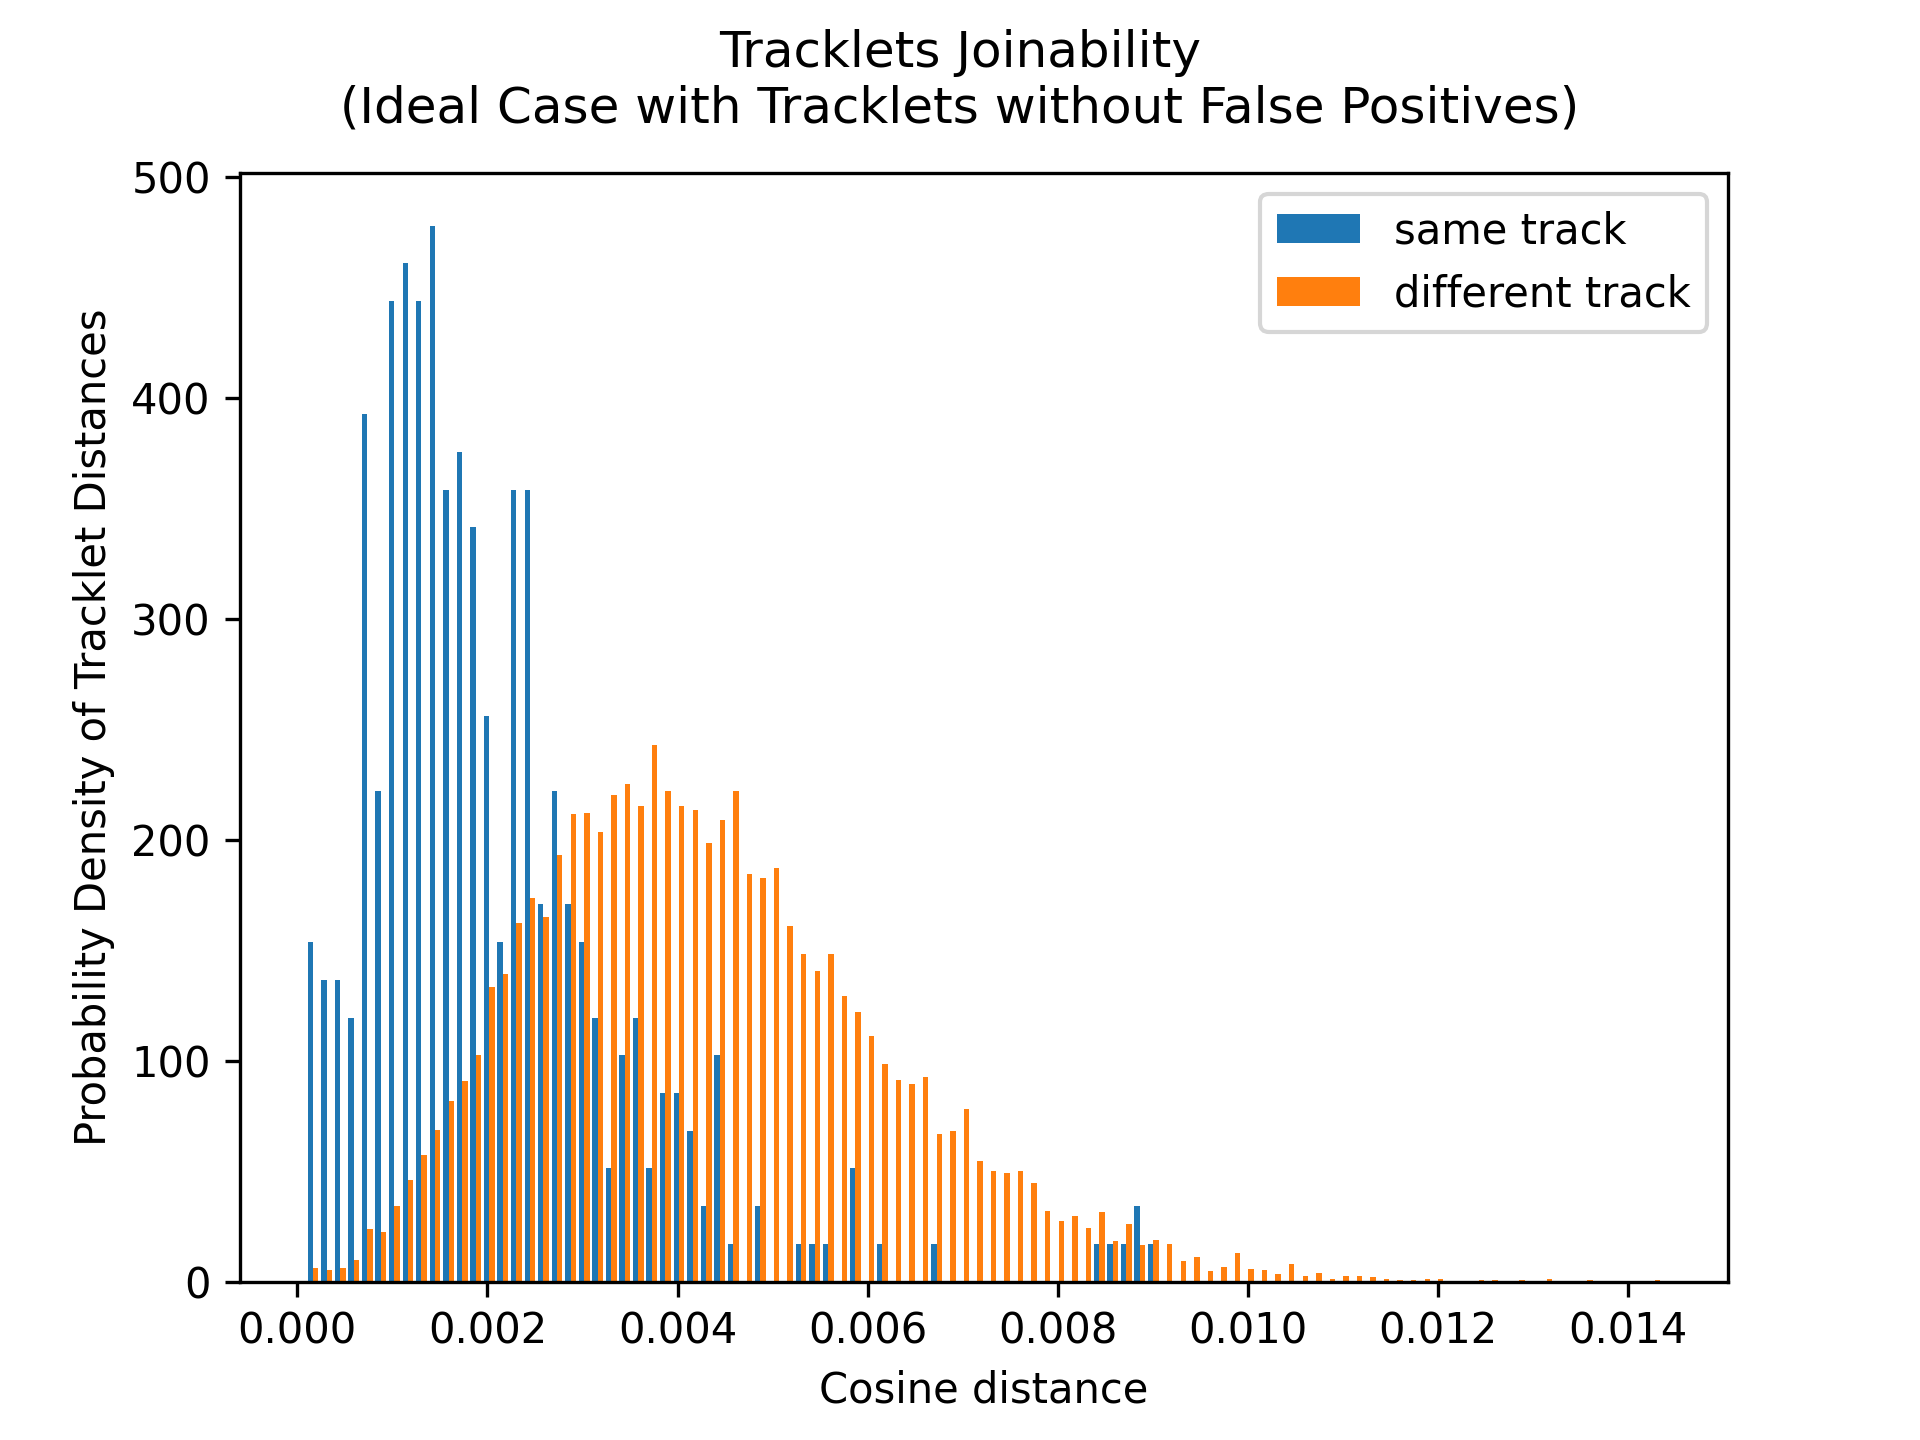
\includegraphics[width=\textwidth]{figures/06_results/atr/03_tracklet_dist_hist.png}
		\caption{\footnotesize{Normalized density function to determine the viability of an appearance model that fuse tracklets by their mean descriptor.}}
		\label{fig:appearance_joinability_all}
	\end{subfigure}
	\begin{subfigure}[]{0.49\textwidth}
		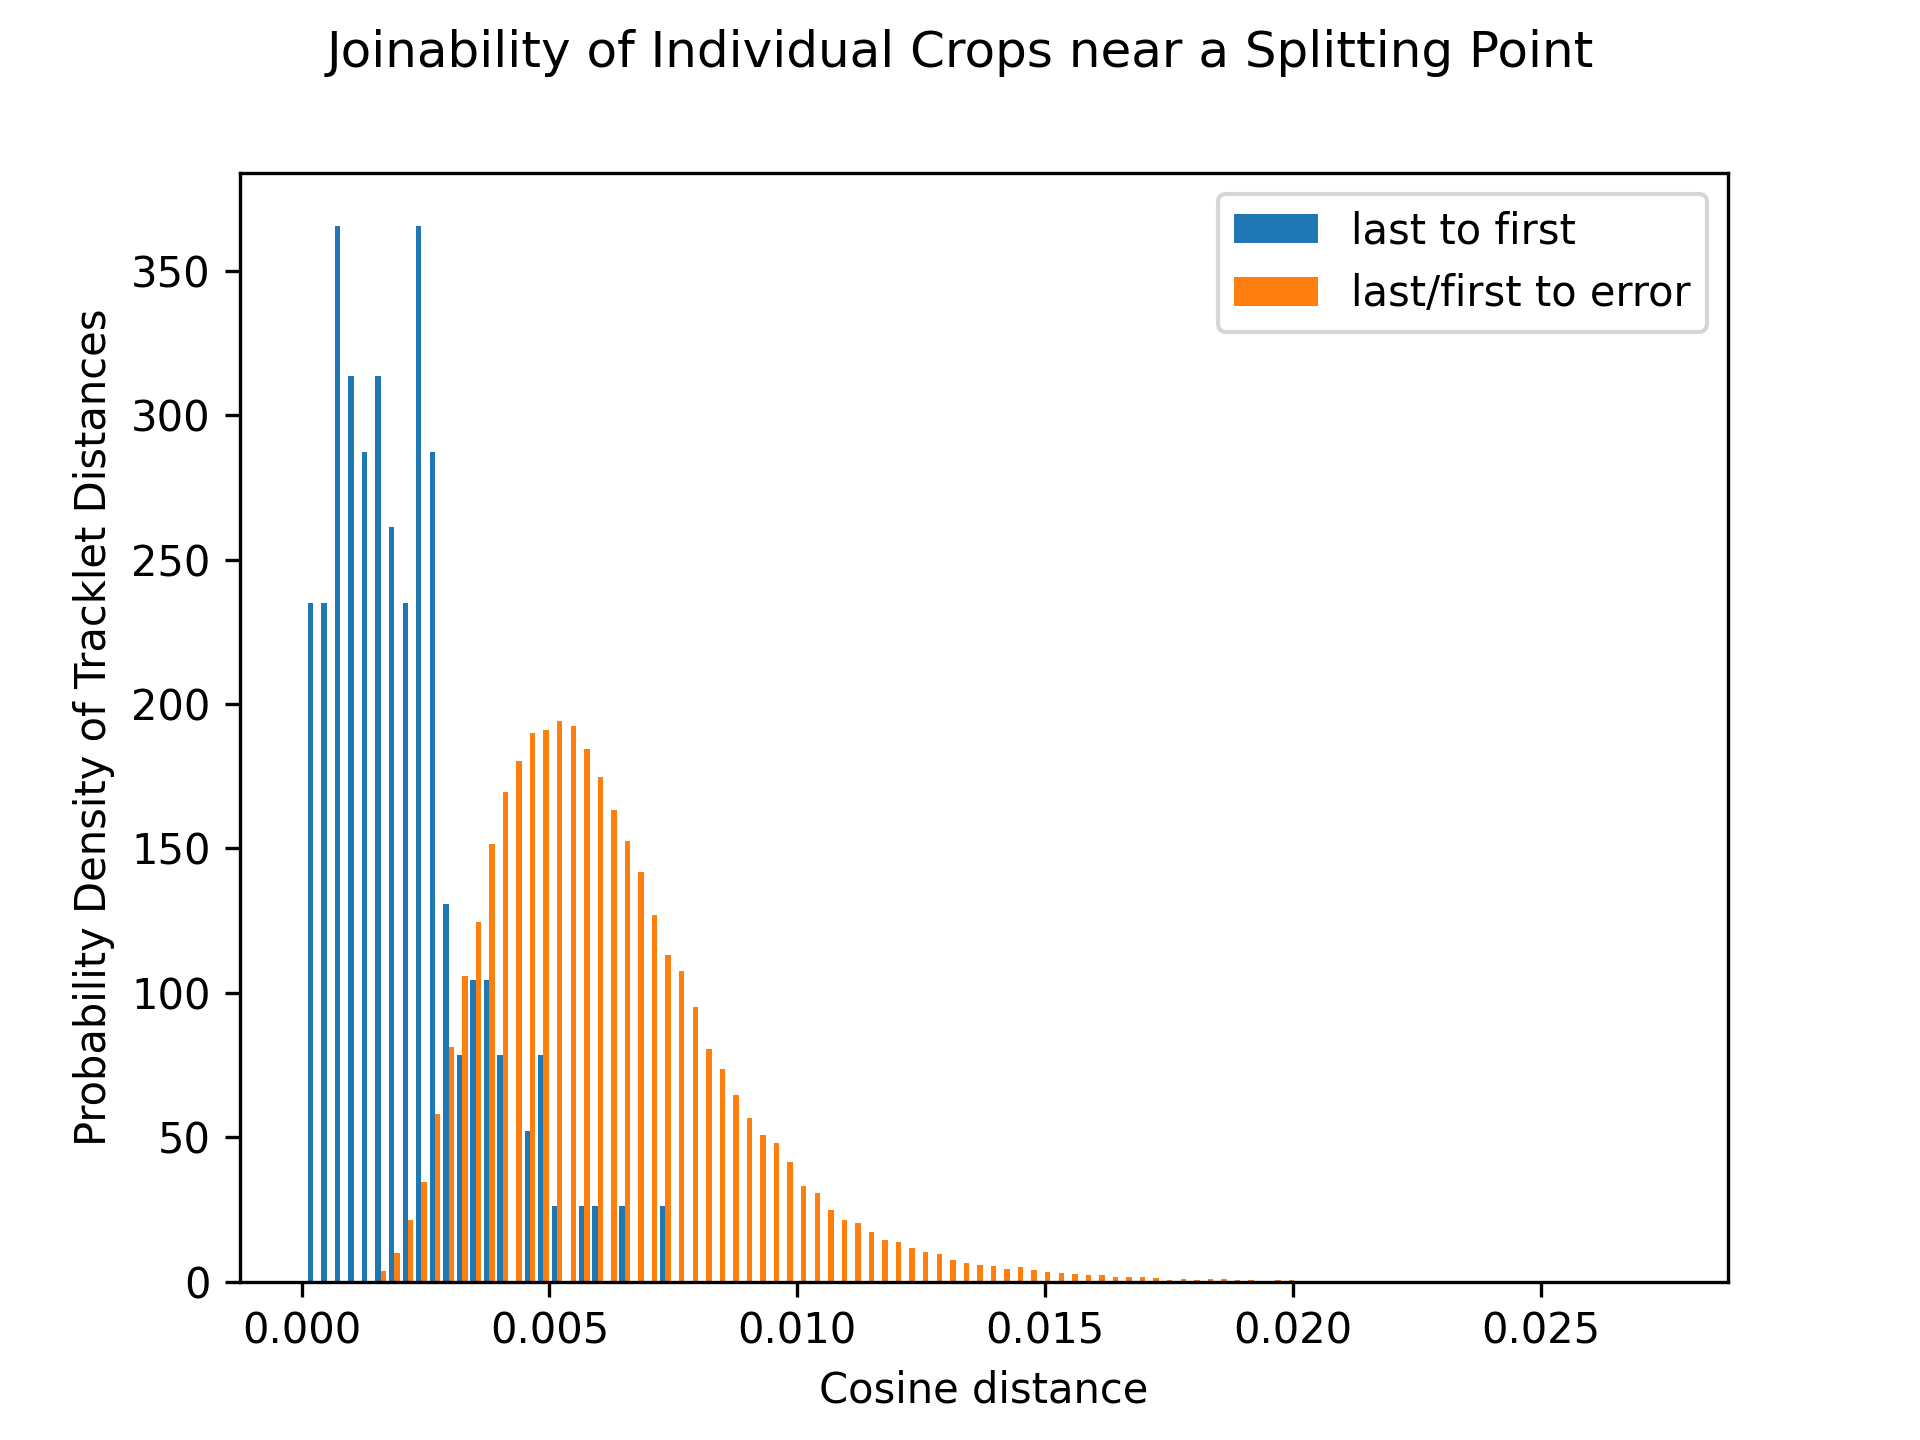
\includegraphics[width=\textwidth]{figures/06_results/atr/05_split_dist_hist.png}
		\caption{\footnotesize{Normalized density function to determine the viability of an appearance model that fuse tracklets based on the last known detection.}}
		\label{fig:appearance_joinability_scope}
	\end{subfigure}
	\caption[Appearance features associability]{\footnotesize{Appearance features associability tests obtained by analysising the ground truth with a split version of itself.}}
	\label{fig:appearance_joinability}
\end{figure}

\begin{figure}[!hp]
    \centering
    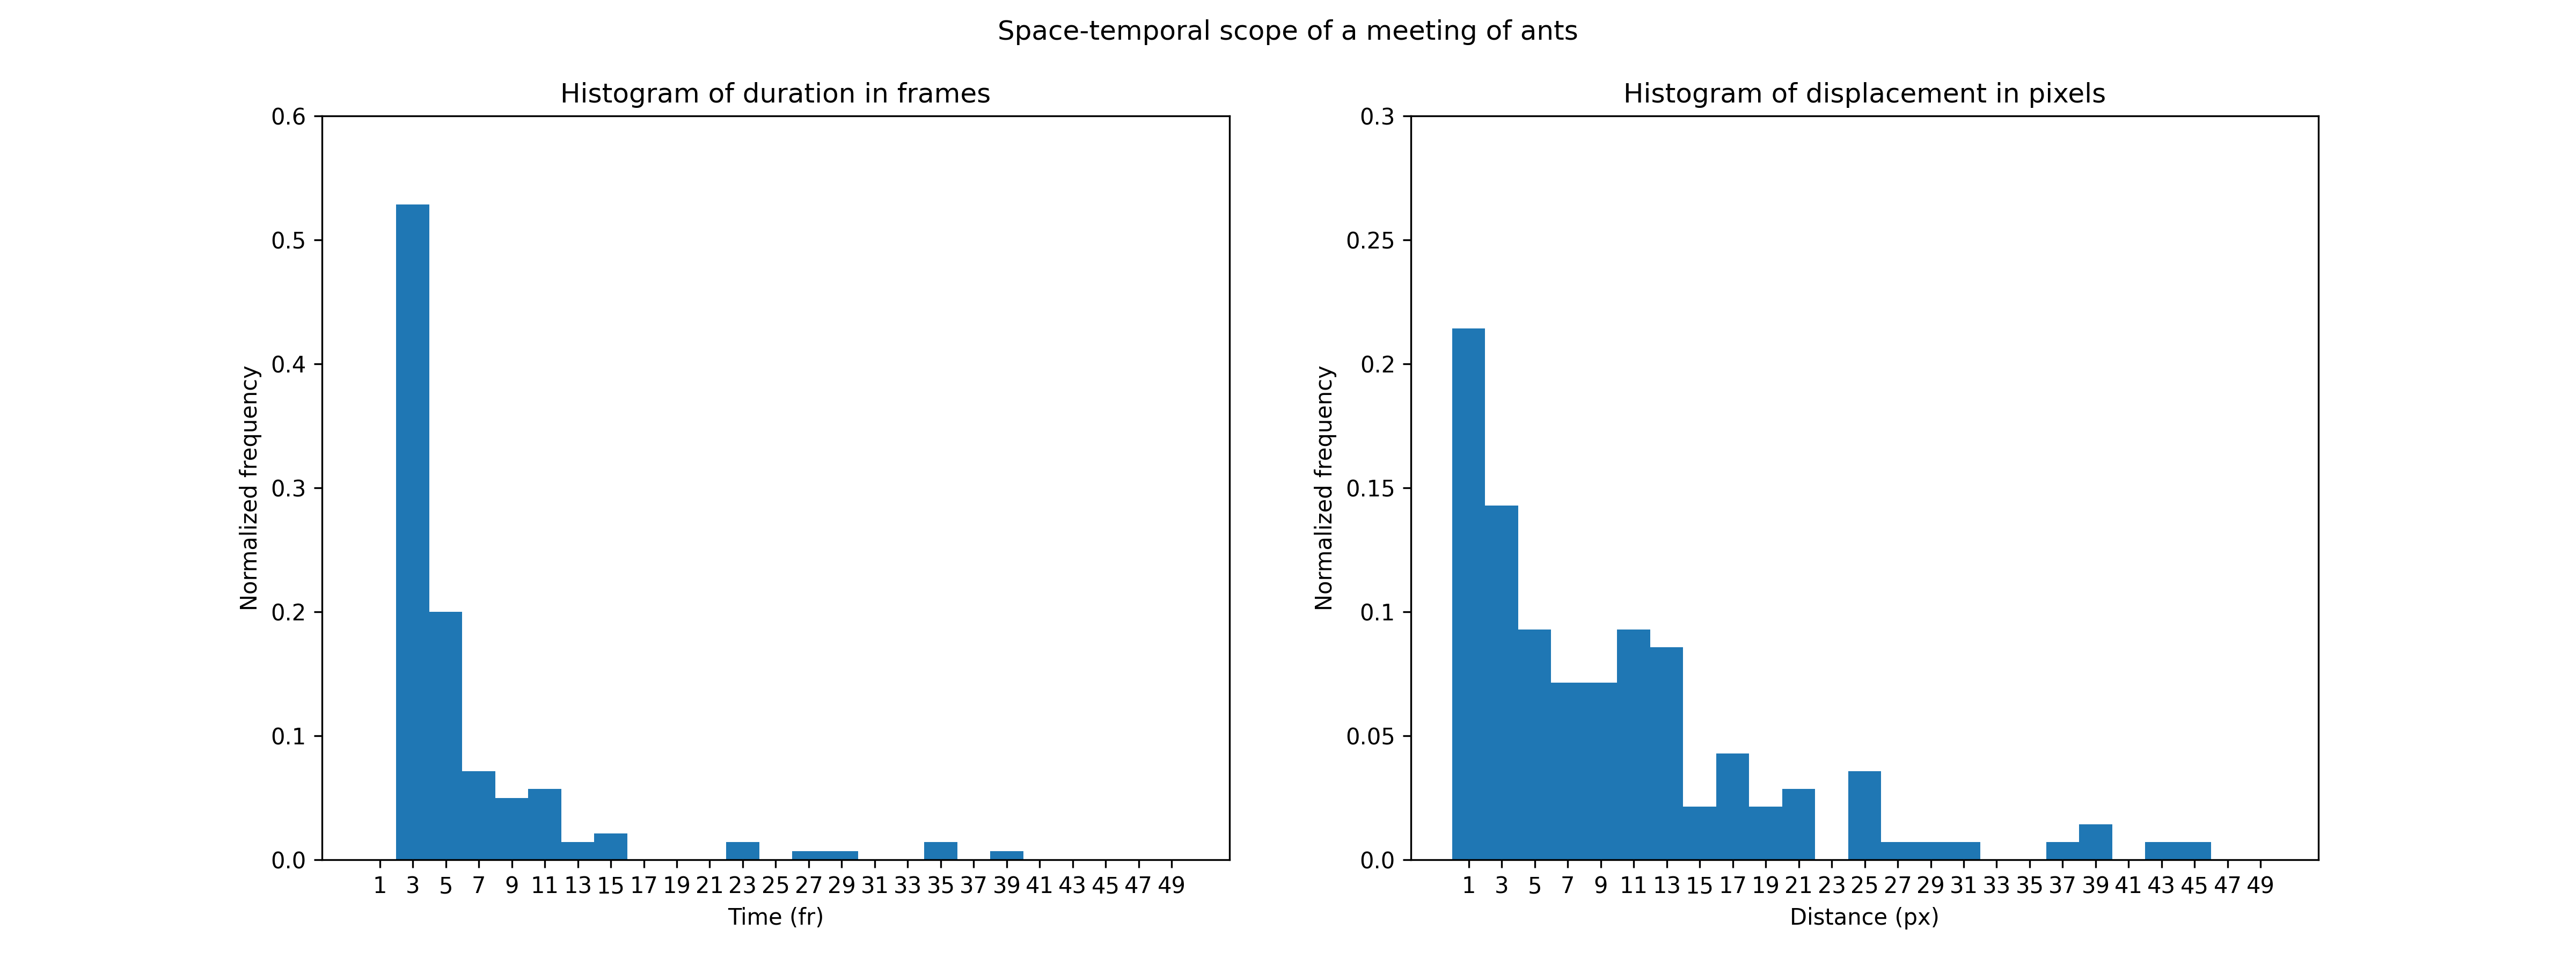
\includegraphics[width=\textwidth]{figures/06_results/atr/04_split_scope_hist.png}
    \caption[Analysis of the occlusions]{\footnotesize{Analysis of the temporal and spatial scope of the occlusions.}}
    \label{fig:occlusion_scope}
\end{figure}

\FloatBarrier

\needspace{0.25\textheight}
\subsection{Tracking Results} 

{
    Finally, after testing the final models, using the different detectors and tracking algorithms, and manually searching for good hyperparameters, the results can be seen on Table \ref{tab:trackers-comparison}.
}

\begin{table}[H]
    \centering
    \caption[Detectors mAP Comparison]{ \footnotesize Comparison of detectors \ac{mAP}, ``Background extraction" is reduced into fgbg.}
    \label{tab:trackers-comparison}

    \begin{tabularx}{\textwidth}{
        @{\hspace{0.001\textwidth}}
        >{\raggedright\arraybackslash}X
        >{\centering\arraybackslash}p{0.1\textwidth}|
        >{\centering\arraybackslash}p{0.1\textwidth}|
        >{\centering\arraybackslash}p{0.1\textwidth}|
        >{\centering\arraybackslash}p{0.1\textwidth}
        @{\hspace{0.001\textwidth}}
    }
        \toprule
        \textbf{Model Name} & \textbf{DetA} & \textbf{LocA} & \textbf{AssA} & \textbf{HOTA} \\
        \midrule
        \midrule
        fgbg - SORT & 20\% & 70\% & 36\% & 27\% \\
        fgbg - OC-SORT & 20\% & 71\% & 40\% & 28\% \\
        yolo - SORT & \textbf{40\%} & 74\% & 61\% & 48\% \\
        yolo - Deep SORT & 08\% & 71\% & 01\% & 03\% \\
        \textbf{yolo - OC-SORT} & \textbf{40\%} & 76\% & 63\% & \textbf{49\%} \\
        yolo - Deep OC-SORT & \textbf{40\%} & 74\% & 62\% & 48\% \\
        \bottomrule
    \end{tabularx}
\end{table}

{
    The usage of the interpolator (\ac{GSI}) did not affect the results, and the \ac{PCA} correction on the ant trajectory slightly deteriorate them.
}

{
    From Table \ref{tab:trackers-comparison} the worse case is the Deep SORT, 
    which only uses appearance to resolve split tracks and fails to associate the observatons, 
    and the best case is the OC-SORT, which discards the appearance model. 
    Additionally, the detector is the component with a strongest influence on the final results.
}

\clearpage

\subsection{Tracking Results analysis}


{
    From Figure \ref{fig:tracks_speed} it can be seen that the tracker predicts faster trajectories than the real ones, 
	however, when observing Figure \ref{fig:tracker_module_diff}, that shows the module difference between the real and predicted velocities, 
	it can be seen the opposite; both ideas can be interpreted together: The tracker correctly tracks most of the fast ants 
	(which may be constantly moving for a certain time), and requires some time to adapt when the ant accelerate or stops 
	(it is the expected behavior of a tracker). Nevertheless, the gross error is small.
}

\begin{figure}[!hp]
	\centering
    \begin{subfigure}[]{0.45\textwidth}
		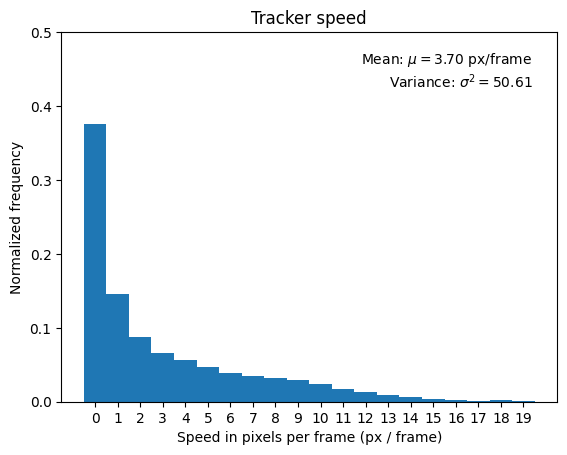
\includegraphics[width=\textwidth]{figures/06_results/da/TrackerSpeed.png}
		\caption{\footnotesize{Probabilistic representation of the speed of the ants within a sequence processed by the best tracker.}}
		\label{fig:tracks_speed_tck}
	\end{subfigure}
	\begin{subfigure}[]{0.45\textwidth}
		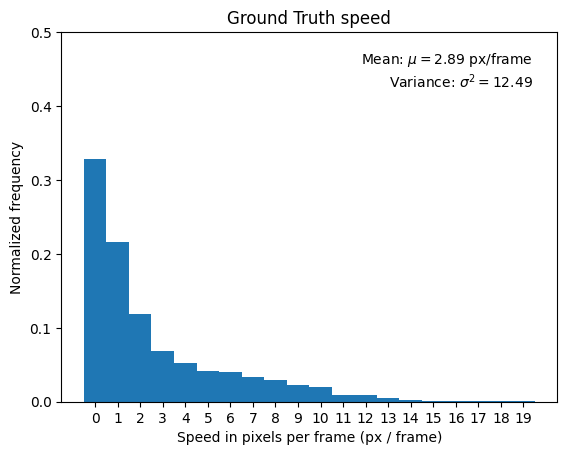
\includegraphics[width=\textwidth]{figures/06_results/da/GroundTruthSpeed.png}
		\caption{\footnotesize{Probabilistic representation of the speed of the ants within a ground truth sequence.}}
		\label{fig:tracks_speed_gt}
	\end{subfigure}
	\caption[Ants speed Normalized histogram]{\footnotesize{Comparison of the probabilistic representation of the speed of the ants between the best tracker and the ground truth.}}
	\label{fig:tracks_speed}
\end{figure}

\begin{figure}[!hp]
    \centering
    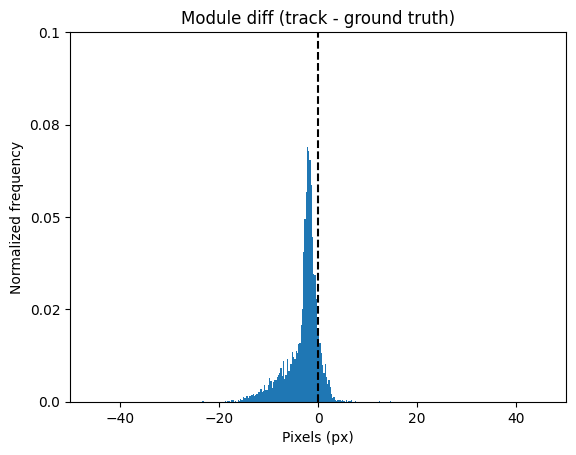
\includegraphics[width=0.45\textwidth]{figures/06_results/da/ModuleDiffTrack.png}
    \caption[Asymmetric error in tracker displacement]{\footnotesize{Asymmetric error in tracker displacement.}}
    \label{fig:tracker_module_diff}
\end{figure}

\needspace{0.1\textheight}

{
	Similar to the velocity, the location metrics computed with two consecutive bounding boxes within a track can be used in the study of the tracking results. 
	The histograms of \ac{IoU} can be seen in Figure \ref{fig:tracks_iou}, 
	comparing the ground truth with the tracker, it can be observed the tracker adapts correctly. 
	The histograms of \ac{CIoU} can be seen in Figure \ref{fig:tracks_ciou}, in these plots, 
	the distribution shifts towards higher scores compared to IoU. 
	The distribution shifts provides a smoother representation of the ground truth, making it easier for the tracker to reproduce the ground truth distribution, by instance, near the score value 1, where the ants are static.
}

\begin{figure}[!hp]
	\centering
	\begin{subfigure}[]{0.9\textwidth}
		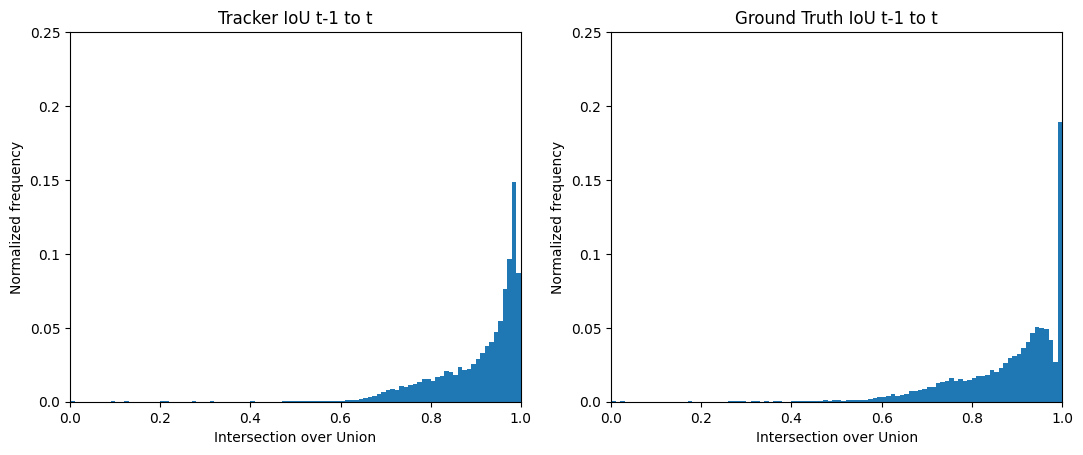
\includegraphics[width=\textwidth]{figures/06_results/da/Tracker_iou_vs_gt.png}
		\caption{\footnotesize{Comparison of the probabilistic representation of the IoU of the ants between the best tracker and the ground truth.}}
		\label{fig:tracks_iou}
	\end{subfigure}
	\begin{subfigure}[]{0.9\textwidth}
		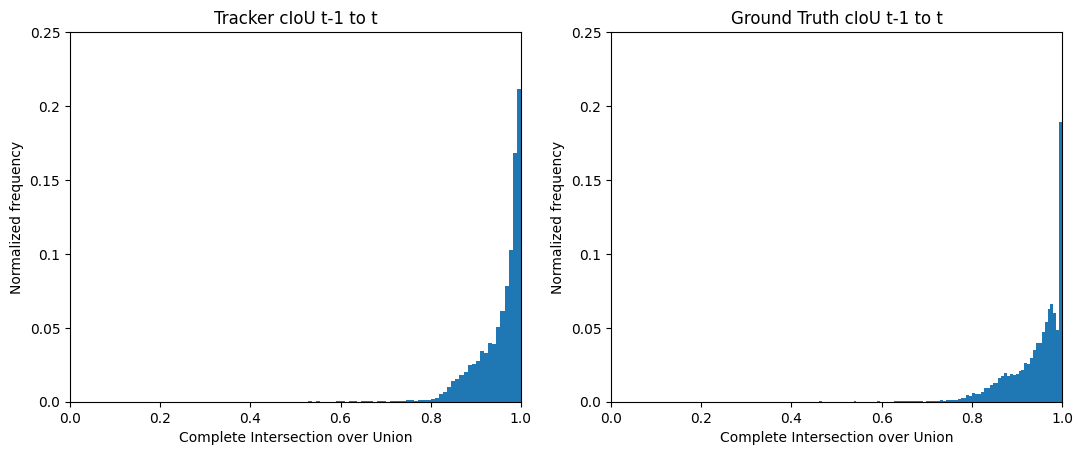
\includegraphics[width=\textwidth]{figures/06_results/da/Tracker_ciou_vs_gt.png}
		\caption{\footnotesize{Comparison of the probabilistic representation of the cIoU of the ants between the best tracker and the ground truth.}}
		\label{fig:tracks_ciou}
	\end{subfigure}
	\caption[Location metrics between frames]{\footnotesize{Comparison of the probabilistic representation of the the locations similarity within a track on the ground truth and the best tracker.}}
	\label{fig:tracks_location}
\end{figure}

\needspace{0.1\textheight}

{
	Figure \ref{fig:tracker_errors} and \ref{fig:tracker_iou_with_gt} were done by associating tracks and ground truth as explained in the HOTA subsection from the methodology section.
}

{
    From Figure \ref{fig:tracker_errors}, the right plot shows that the angular error of the estimated displacement is small, 
	a good explanation for the unsuccessful PCA model: adding complexity when it works will become a noisy source. 
	The left plot shows the module error of the estimated displacement is small, more detailed characterization was done at the beginning of this subsection (using module difference instead of module error).
}

{
	Figure \ref{fig:tracker_iou_with_gt} depicts the IoU of associated tracks and ground truth, 
	it is noticiable the valley at 0.8 IoU, which divides the data of a plot approximately in a 40\% at the left and a 60\% at the right. 
	Coinciding with the 60\% \ac{AssA} which measures the correct associations of observations and tracks.
}


\begin{figure}[!hp]
    \centering
    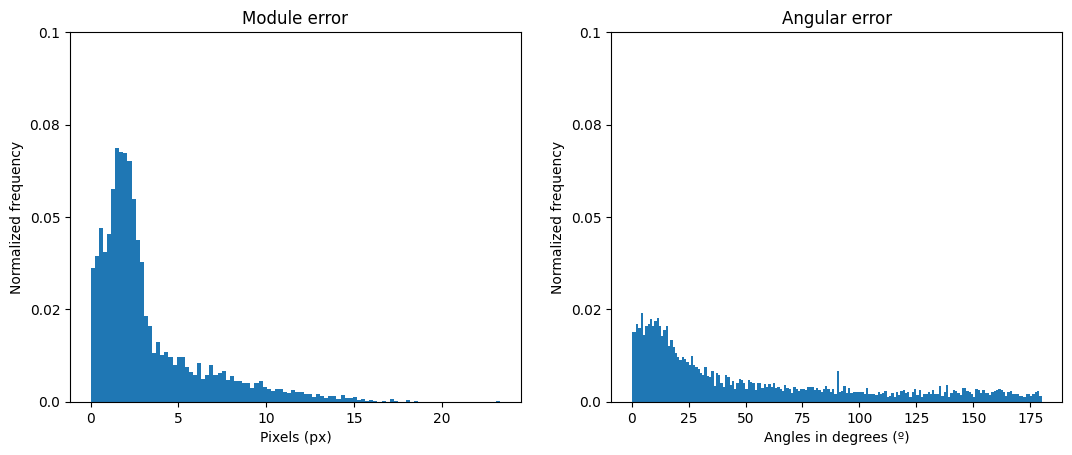
\includegraphics[width=0.9\textwidth]{figures/06_results/da/TrackerError.png}
    \caption[Displacement and angular error of the best tracker]{\footnotesize{The error in distance and angle of the best tracker.}}
    \label{fig:tracker_errors}
\end{figure}

\begin{figure}[!hp]
    \centering
    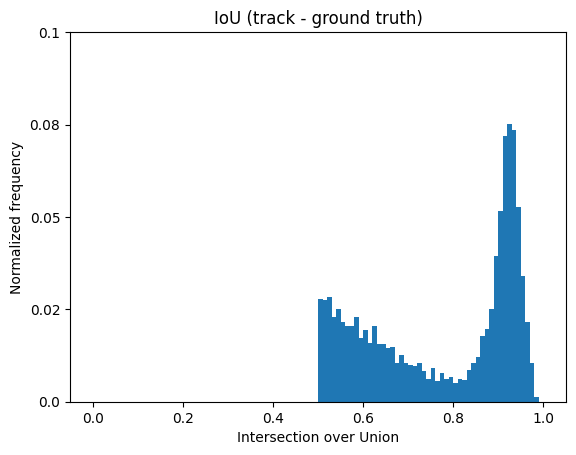
\includegraphics[width=0.45\textwidth]{figures/06_results/da/TrackerIoU_GT.png}
    \caption[Location similarity between the best tracking and the ground truth]{\footnotesize{Location similarity between the best tracking and the ground truth}}
    \label{fig:tracker_iou_with_gt}
\end{figure}

\FloatBarrier

%{
%    Finally, the HOTA metric is depicted in the Figure \ref{fig:tracker_hota_alpha}, 
%	and a 2D representation of a tracked sequence compared with its ground truth is shown in Figure \ref{fig:OCSORT_performance}, 
%	where each color line is a track and each row is a different identity.
%}
%
%\begin{figure}[!p]
%    \centering
%    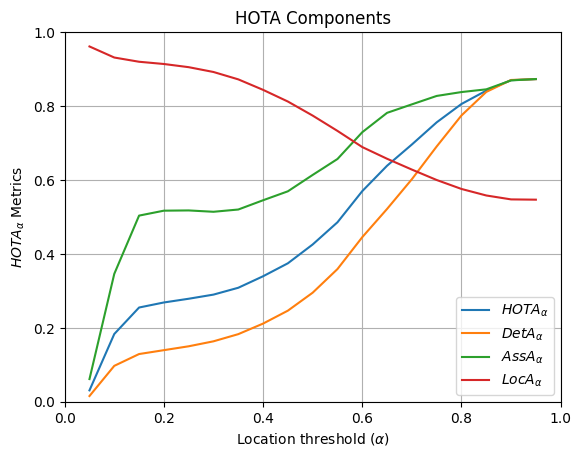
\includegraphics[width=0.9\textwidth]{figures/06_results/HOTA_componens.png}
%    \caption[Best tracker HOTA]{\footnotesize{HOTA partial components in function of the threshold for the best tracker.}}
%    \label{fig:tracker_hota_alpha}
%\end{figure}
%
%\begin{figure}[!p]
%	\centering
%	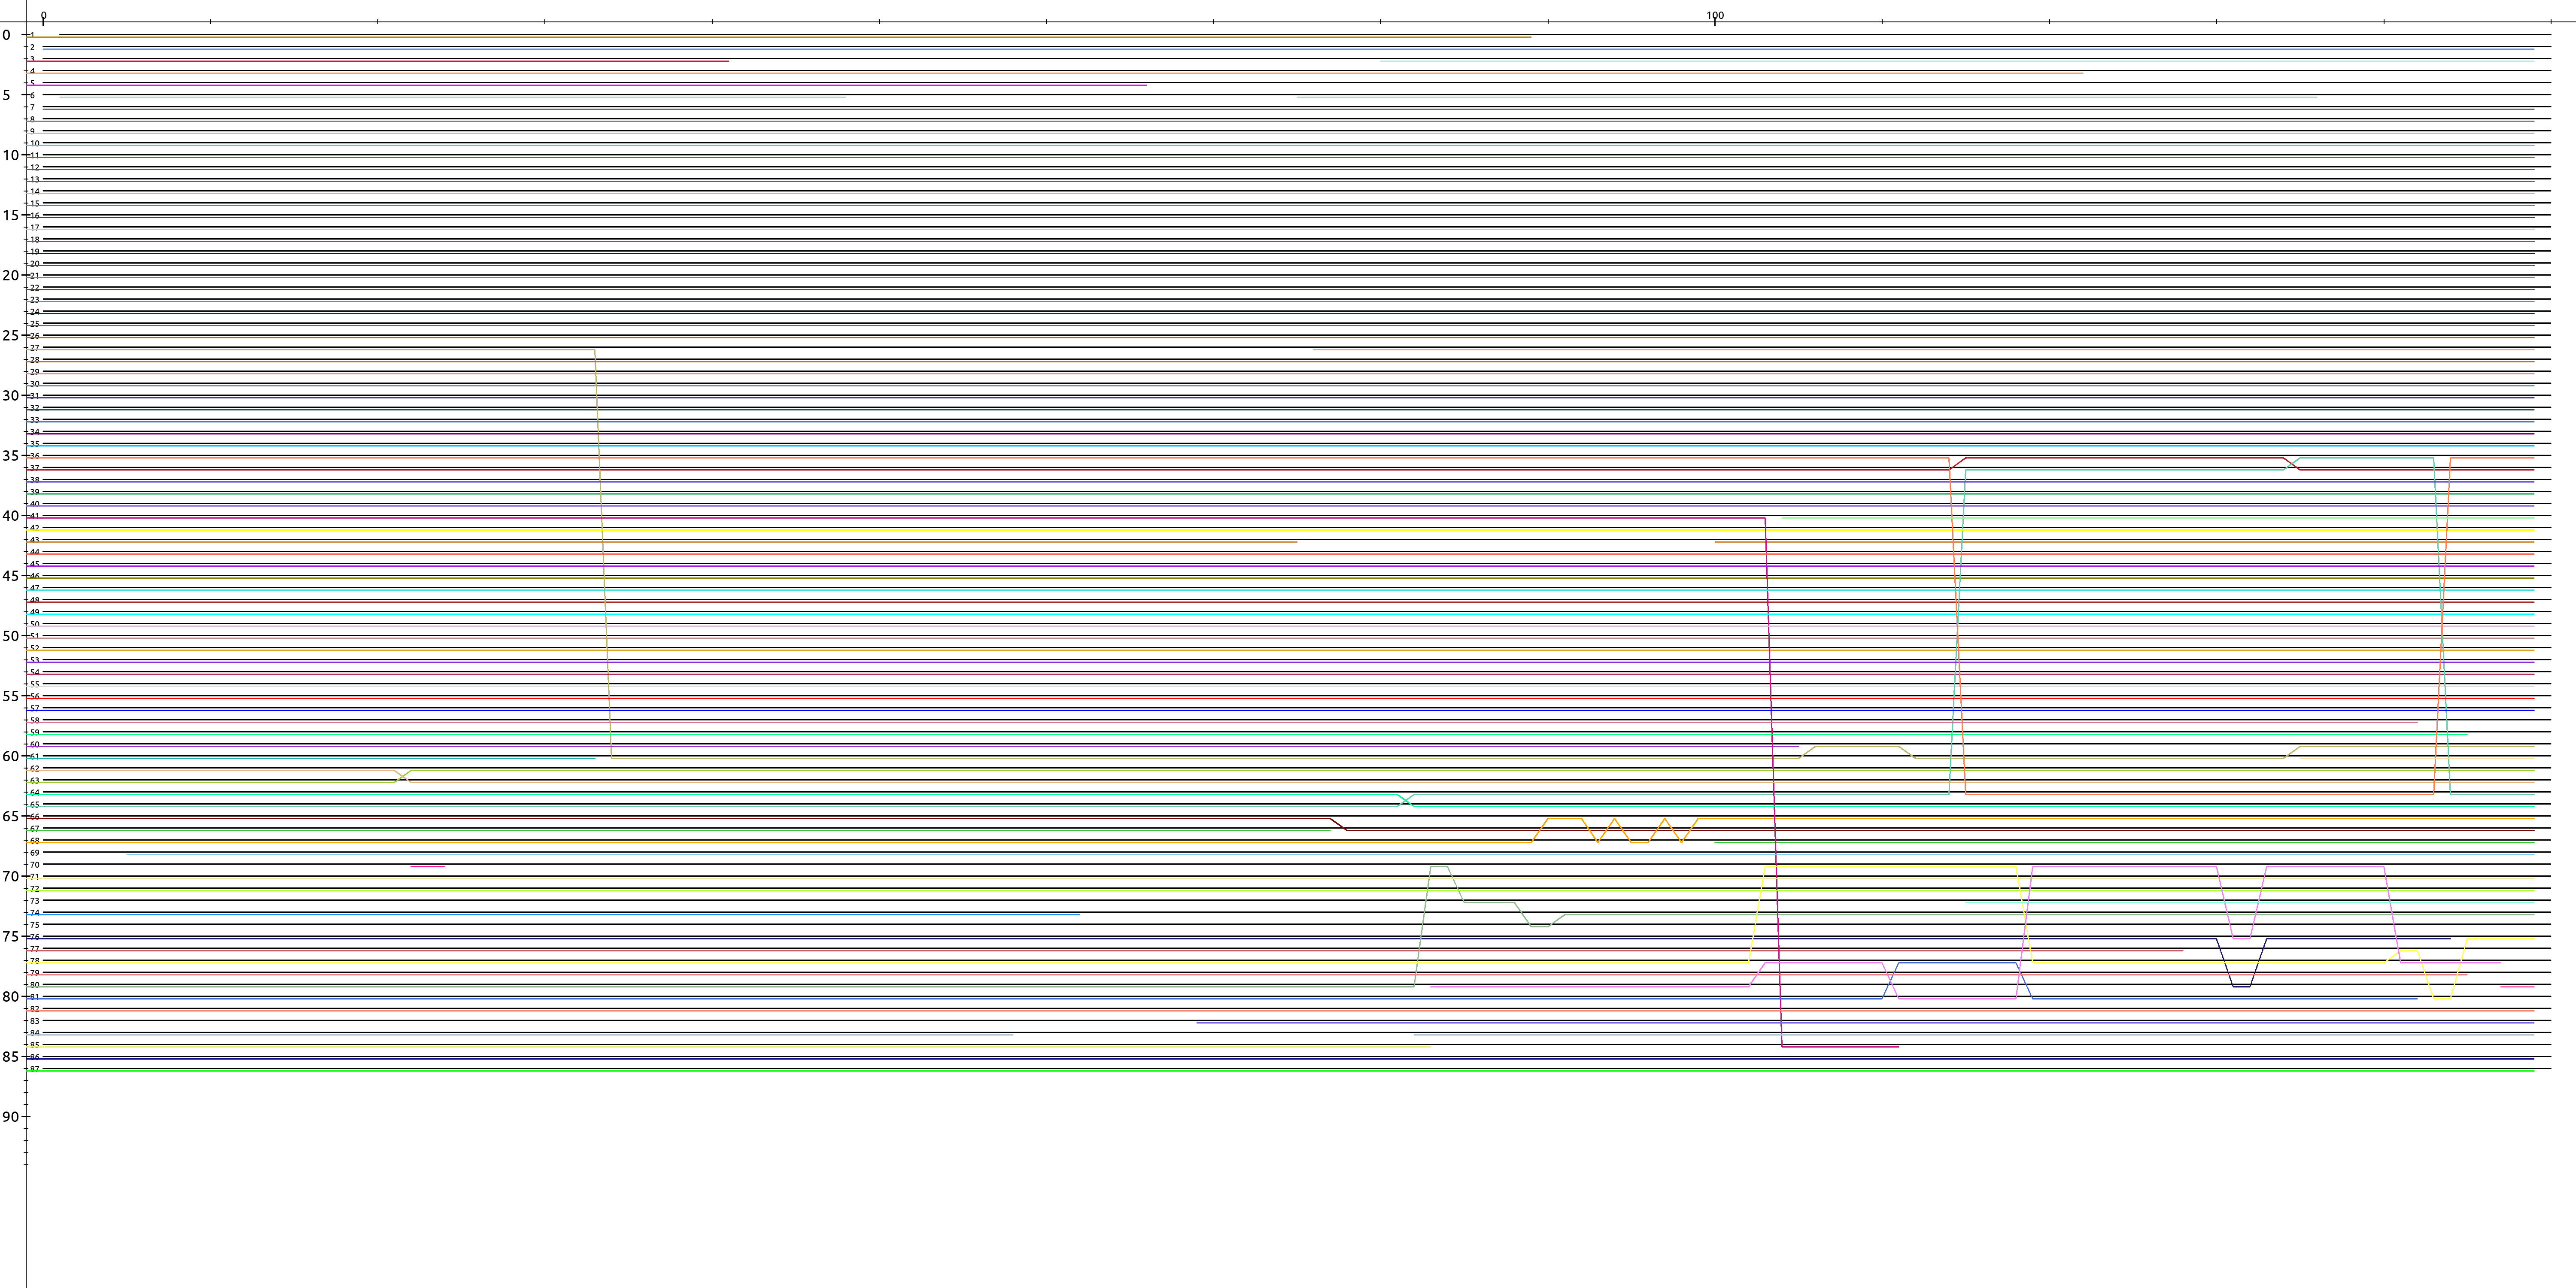
\includegraphics[width=0.9\textwidth]{figures/06_results/da/ocsort-results.png}
%	\caption[Visual representation of the OCSORT results]{\footnotesize{Visual representation of the OCSORT results.}}
%	\label{fig:OCSORT_performance}
%\end{figure}

\FloatBarrier
